\documentclass[14pt, a4paper] {ncc}
\usepackage[utf8] {inputenc}
\usepackage[T2A]{fontenc}
\usepackage[english, russian] {babel}
\usepackage[top=20mm, bottom=20mm, left=25mm, right=10mm]{geometry}

% Чтобы зачёркивать символы
\usepackage[makeroom]{cancel}

\usepackage{xcolor}
\usepackage{tikz}

\usepackage{biblatex}

% Для вставки фигур
\usepackage{float}
\usepackage{caption}


\usepackage{longtable,amsmath,amsfonts,amssymb}

\usepackage{listings}
\usepackage{algpseudocode}
% More Math Symbols
\usepackage{stmaryrd}

% Enumeration
\usepackage{enumitem}
\setlist[enumerate]{topsep=0pt,itemsep=0ex,partopsep=1ex,parsep=1ex}
\setlist[itemize]{itemsep=0ex}

% Полуторный межстрочный интервал
\usepackage[nodisplayskipstretch]{setspace}
\onehalfspacing

% Добавить абзацный отступ для первых абзацев в section/subsection,
% по умолчанию не добавляется
\usepackage{indentfirst}

% Красивый маркер ненумерованного списка в виде тире
\def\labelitemi{--}

% Times New Roman
\usepackage{pscyr}
\renewcommand{\rmdefault}{ftm}


% Абзацный отступ равен 1.25 см
\parindent=1.25cm

% Номер страницы по середине верхнего поля
\usepackage{fancyhdr}
\pagestyle{fancy}
\fancyhf{}
\fancyhead[C]{\thepage}
\renewcommand{\headrulewidth}{0pt}

\addto\captionsrussian{
% "Оглавление" вместо "Содержание"
  \def\figurename{{Оглавление}}
% подпись "Рисунок" вместо "Рис"
  \def\figurename{{Рисунок}}
}

% Каждый пункт оглавления должен быть с отточием
\usepackage{titletoc}
% Максимальная вложенность содержания (только разделы, подразделы и
% "пункты")
\setcounter{tocdepth}{3}

% Возможность переопределять оглавление и его стиль
\usepackage{tocloft}
% Слово "Оглавление" заглавными буквами
\makeatletter
\patchcmd{\@cftmaketoctitle}{\cfttoctitlefont\contentsname}{\cfttoctitlefont\MakeUppercase{\contentsname}}{}{}
\makeatother

% Самое длинное тире в качестве разделителя в подписях к рисункам,
% таблицам, листингам и др.
\usepackage{caption}
\DeclareCaptionLabelSeparator{emdash}{ --- }
\captionsetup{labelsep=emdash}

% Подпись к таблице должна быть по левому краю
\captionsetup[table]{singlelinecheck=false}

% Сквозная нумерация таблиц, формул, рисунков
%\renewcommand{\theequation}{\arabic{equation}}
%\renewcommand{\thetable}{\arabic{table}}
%\renewcommand{\thefigure}{\arabic{figure}}


% Обязательно переносить слова, чтобы соблюсти поля документа. Для
% соблюдения полей можно пренебречь правилами для тех слов и
% словосочетаний, о которых не знают словаря переносов (ruhyphen или
% ruenhyph). Оно почему-то работает. Взято с:
%
%   http://www.latex-community.org/forum/viewtopic.php?p=70342#p70342
%
\tolerance 1414
\hbadness 1414
\emergencystretch 1.5em
\hfuzz 0.3pt
\widowpenalty=10000
\vfuzz \hfuzz
\raggedbottom

%%%%%%%%%%%%%%%%%%%%%%%%%
\lstdefinelanguage{MyLang}
{
  morekeywords={data},
  keywordstyle=\bfseries\color{black}
}

\lstset{language=Haskell}
\lstset {
mathescape,extendedchars=\true,frame=single,basicstyle=\ttfamily
}

%%%%%%%%%%%%%%%%%%%%%%%%%
\newcommand{\larrow}{\leftarrow}
\newcommand{\rarrow}{\rightarrow}

\newcommand{\embed}{\unlhd}
\newcommand{\inst}{\preccurlyeq}
\newcommand{\strictinst}{\prec}
\newcommand{\ukanren}{$\mu$Kanren }

\newcommand{\origin}[1]{(англ. {\it #1})}

\newcommand{\rel}[1]{$\text{#1}^o$}

\newcommand{\todo}[1]{{\bf\color{red}TODO: #1}}
%%%%%%%%%%%%%%%%%%%%%%%%%

\addbibresource{main.bib}

\begin{document}
\setcounter{figure}{0}

%\tableofcontents
%\newpage
%\section{Введение}

%\newpage
\section{Описание предметной области}

\subsection{Логическое и реляционное программирование}

{\bf Логическое программирование}~--- это вид декларативного программирования,
основанный на формальной логике. Программы представляются в виде
утверждений, представляющихся логическими формулами и описывающих
определённую область проблем.
``Вычисление'' программы в контексте логического программирования производится
в форме \emph{поиска} доказательства утверждений на основе заданных
фактов --- аксиом --- и правил вывода в соответствии с заданной
\emph{стратегией поиска}~\cite{logicMJ}.

Стратегия поиска задаёт,
каким образом происходит обход пространства поиска ответов, и,
как следствие, определяет как, какие и в каком порядке будут находиться
ответы. Стратегия поиска, при которой каждый возможный ответ будет со временем
выдан, называется \emph{полной}. Чаще применяются \emph{неполные} стратегии,
поскольку они менее требовательны к вычислительным ресурсам~\cite{currySearch}.

Самые известные языки логического программирования --- языки семейства Prolog.
Prolog применяется для доказательства теорем~\cite{prologTheorem},
проектирования баз знаний, создания экспертных систем~\cite{prologExSys}
и искусственного интеллекта~\cite{prologInt}.
Prolog строится на логике предикатов первого порядка в форме дизъюнктов
Хорна (то есть дизъюнктов только с одним положительным литералом) и
использует \emph{метод резолюций}, основанный на доказательстве от
противного, для решения задач.
Prolog вводит разнообразные синтаксические конструкции с
\emph{побочными эффектами}, то есть с действиями, приводящими к изменению
\emph{окружения} программы, к примеру, оперaтор отсечения~\origin{cut},
который влияет на способ вычисления программы, предотвращая нежелательные
вычисления.
Также он использует стратегию обхода в глубину, что приводит к тому, что
поиск может ``зациклиться'' и никогда не выдать оставшиеся решения,
но, тем не менее, благодаря своим расширениям Prolog
остаётся хорошим решением для задач из своей области применения~\cite{logicMJ}.

% Подобные операторы обычно используются для того, чтобы
% повысить эффективность программ, однако 

% Другие языки логического программровани, такие как Mercury\cite{mercury} или 
% Curry\cite{curry}, являются 

% {\bf Логическое программирование}~--- это вид декларативного программирования,
% основанный на логике предикатов первого порядка в форме дизъюнктов Хорна
% (то есть дизъюнктов
% с только одним положительным литералом),
% применяющий принципы логического вывода на основе заданных фактов и правил.
% Программа, написанная на логическом языке --- это множество логических формул,
% описывающих определённую область проблем.\cite{logicMJ}

% Существует множество языков логического программирования, таких как Prolog, Curry, Mercurry,
% однако самые известные --- языки семейства Prolog. Prolog применяется для доказательства
% теорем, проектирования баз знаний, создания экспертных систем и искусственного интеллекта.

% Prolog построен на \emph{методе резолюций}, который является обобщением метода
% ``доказательства от противного'', а в частности --- на \emph{линейном} методе
% резолюций \origin{Linear resolution with Selection function for Definition clauses}.
% При вычислении программы правило резолюции применяется не к случайных дизъюнктам,
% а в строго установленном порядке. В случае, когда вычисления дизъюнкта прошло
% неудачно, происходит \emph{откат} к прошлому состоянию программы, на котором
% выбирался неудавшийся дизъюнкт\cite{logicMJ}.
% 
% Помимо этого, Prolog вводит разнообразные синтаксические конструкции с побочными \emph{эффектами},
% то есть с действиями, приводящими к изменению \emph{окружения} программы,
% к примеру, оперaтор отсечения~\origin{cut},
% который влияет на способ вычисления программы.

% Это свойства определяют Prolog как язык, однако из-за них теряется свойство \emph{реляционности}.

% % 
% % Пример программы на Prolog приведён в Листинге~\ref{lst:memberProlog}.
% % 
% % \begin{lstlisting}[language=Prolog,caption={Проверка принадлежности элемента списку},captionpos=b,label={lst:memberProlog}]
% % member(X, [X | T]).
% % member(X, [H | T]) :- member(X, T).
% % \end{lstlisting}
% % 
% % В этой программе проверяется принадлежность элемента списку. Есть два возможных
% % варианта происходящего: либо элемент равен элементу в голове списка




{\bf Реляционное программирование}~--- это форма чистого логического
программирования, в котором программы задаются как набор
математических {\it отношений}. Реляционное программирование направлено
на получение \emph{значимых} ответов, как бы ни использовались отношения
~\cite{byrdMK}.

Исторически, понятие реляционного программирования появилось
раньше~\cite{relML} и задавало саму концепцию программы как отношения,
когда логическое --- появилось позже и предоставляло реализацию его
идей~\cite{logicMJ}.
Однако в данной работе под реляционным программированием понимается
непосредственно так, как указано выше.

В терминах реляционного программирования, к примеру, сложение $X + Y = Z$
может быть выражено отношением\footnote{Символ $\ ^o$ традиционно
используется для обозначения отношения.}
\[\text{add}^o (X, Y, Z),\]
которое в зависимости от того, какие переменные заданы, порождает
все возможные значения переменных, при которых отношение выполняется:
\begin{itemize}
\item \rel{add}(1, 2, 3) --- проверка выполнимости отношения;
\item \rel{add}(1, 2, A) --- поиск всех таких A, при которых 1 + 2 = A;
\item \rel{add}(A, B, 3) --- поиск всех таких A и B, при которых A + B = 3;
\item \rel{add}(A, B, C) --- поиск всех троек A, B и С, при которых A + B = C.
\end{itemize}

Чистые отношения не предполагают функциональных зависимостей между переменными,
поэтому поиск можно проводить в разных ``направлениях'', в зависимости от
того, какие переменные заданы, как показано выше в примере.

Когда же отношения вырождаются в функциональные и появляется
явная зависимость между переменными, тогда можно говорить про запуск
в ``прямом'' направлении --- то есть задаются входные аргументы --- и в
``обратном'' --- при задании результата.

К примеру, отношение ``меньше'' для двух чисел X и Y можно задавать как
\rel{less}(X, Y) и получить чистое реляционное отношение, либо
как \rel{$\text{less}_2$}(X, Y, R), где R сообщает, состоят ли X и Y
в отношении, и получить функциональное, и тогда задание X и Y будет
прямым направлением, а задание R --- обратным.

% Отличительная черта реляционного программирования в том, что с каким бы
% набором аргументов отношение ни было запущено, обязательно должны быть
% найдены все ответы, если они есть. Для сравнения, в Prolog 

% Ссылка на Булычева
Одно из применений реляционной парадигмы --- {\it реляционные интерпретаторы}.
Для языка $L$ его интерпретатор -- это функция $\text{eval}_L$, которая принимает
на вход программу $p_L$ на этом языке, её вход $i$ и возвращает некоторый выход $o$:
\[ \text{eval}_L (p_L, i) \equiv \llbracket p_L \rrbracket (i) = o \]
Реляционную версию интерпретатора можно представить как отношение:
\[ \text{eval}_L^o(p_L, i, o). \]

При запуске такого отношения в разных направлениях можно добиться интересных
эффектов: не только вычислять результат, но и по программе $p_L$ и выходу $o$
искать возможные входы $i$ или вовсе генерировать программу по указанным
выходам и входам.
% решать задачи поиска по задаче распознавания~\cite{lozov},
%генерировать программы по заданной спецификации входа $i$ и выхода $o$~\cite{unifiedMK}.

Можно отметить, что языках, основанных на классическом Prolog, производить
подобные вычисления для получения вразумительных результатов не получится. 


\subsubsection{miniKanren}

% Byrd
{\it miniKanren} -- семейство встраиваемых предметно-ориентированных языков,
специально спроектированное для реляционного программирования~\cite{byrdMK}.

Основная реализация miniKanren написана на языке Scheme~\cite{reasonedSchemer},
однако существует множество реализаций в ряде других языков, в том числе
Clojure, OCaml, Haskell и другие\footnote{\url{minikanren.org}}.

miniKanren предоставляет набор базовых конструкций: унификация ($\equiv$),
конъюнкция $(\land)$, дизъюнкция $(\lor)$, введение свежей переменной
(\lstinline{fresh}), вызов реляционного отношения,
--- представляющий ядро языка, и разнообразные расширения, к примеру, оператор неэквивалентности
\origin{disequality constraint} или нечистые операторы, предоставляющие функциональность
отсечения из Prolog. Несмотря на то, что в miniKanren введены операторы с эффектами, использование
его только с чистыми операторами предоставляет настоящую реляционность.

Классический пример --- программа конкатенации двух списков --- указан
на рисунке~\ref{fig:appendo}.

\begin{figure}[h!]
\begin{lstlisting}[mathescape,language=Haskell,extendedchars=\true,frame=single,basicstyle=\ttfamily]
$\text{append}^o$ X Y R =
  X $\equiv$ [] $\land$ Y $\equiv$ R $\lor$
  fresh (H X' R')
    (X $\equiv$ H :: X') $\land$
    (R $\equiv$ H :: R') $\land$
    $\text{appendo}^o$ X' Y R'
\end{lstlisting}

\caption{Пример программы на miniKanren (\lstinline{::} --- конструктор списка)}
\label{fig:appendo}
\end{figure}

Пояснение к программе:
список \lstinline{R} является конкатенацией списков \lstinline{X} и
\lstinline{Y} в случае, когда список \lstinline{X} пуст, а \lstinline{Y}
равен \lstinline{R}, либо когда \lstinline{X} и \lstinline{R} раскладываются
на голову и хвост, а их хвосты состоят в отношении конкатенации с \lstinline{Y}.

Для выполнения конкатенации над списками необходимо сформировать
\emph{запрос}~(или \emph{цель}).
В запросе в аргументах указываются либо замкнутые термы, либо термы
со свободными переменными. Результатом выполнения является список
подстановок для свободных переменных, при которых отношение выполняется;
когда свободных переменных нет, подстановка, соответственно, пустая.

На рисунке~\ref{fig:appendoExample} приведёт пример запроса, в котором мы хотим
найти возможные значения переменных \lstinline{Y} и \lstinline{R}. Потенциально
может быть бесконечное число ответов, к примеру, когда все аргументы в запросе
--- переменные, поэтому в системах miniKanren есть возможность запрашивать
несколько первых ответов; в примере, это число 1. Ответы могут содержать в себе
как конкретные замкнутые термы (к примеру, числа), так и свободные переменные,
которые в примере обозначаются как $\text{\_.}_n$. В примере одна и также
свободная переменная $\text{\_.}_0$ назначена и \lstinline{Y} и \lstinline{R}.
Это означает, что какое бы ни было значение \lstinline{Y}, оно всегда будет
являться хвостом \lstinline{R}.

\begin{figure}[h!]
\begin{lstlisting}[mathescape,language=Haskell,extendedchars=\true,frame=single,basicstyle=\ttfamily]
> run 1 (Y R) ($\text{append}^o$ [1, 2] Y R)
Y = $\text{\_.}_0$
R = 1 :: 2 :: $\text{\_.}_0$
\end{lstlisting}
\caption{Пример запуска отношения конкатенации.}
\label{fig:appendoExample}
\end{figure}

В определение miniKanren входит особый алгоритм поиска ответов --- чередующийся
поиск \origin{interleaving search}, основанный на поиске в глубину,
который рассматривает всё пространство поиска и является
полным~\cite{interleaving}.
% гарантирует, что если существует ответ, то алгоритм его предоставит за конечное время\cite{interleaving}.
%Для сравнения, обычный поиск в глубину, используемый в классическом Prolog при методе резолюций, может зациклиться
%или разойтись перед тем, как предоставить все ответы.
Это свойство чередующегося поиска определяет, вместе с отсутствием
нечистых расширений, реляционность miniKanren. 

% Применимость
Хотя miniKanren уже применяется в индустрии для поиска лечения редких
генетических заболеваний в точной медицине~\cite{medMK},
на данном этапе своего развития используется в основном в исследовательских
целях:
\begin{itemize}
\item реляционные интерпретаторы на miniKanren для решения задач поиска~\cite{lozov},
      техника программирования по примерам~\cite{unifiedMK};
\item для доказательство теорем~\cite{mkProver} ;
\item в области вычислительной лингвистики~\cite{mkLing}.
\end{itemize}

%Одно из интересных применений miniKanren --- {\it реляционные интерпретаторы}.
%Для языка $L$ его интерпретатор -- это функция $\text{eval}_L$, которая принимает
%на вход программу $p_L$ на этом языке, её вход $i$ и возвращает некоторый выход $o$:
%\[ \text{eval}_L (p_L, i) \equiv \llbracket p_L \rrbracket (i) = o,\]
%где $\llbracket \bullet \rrbracket $ --- семантика языка L.
%Тогда в miniKanren интерпретатор описывается отношением $\text{eval}^o_L(p_L, i, o)$.
%При запуске такого отношения на разном наборе аргументов можно добиться интересных эффектов:
%\begin{itemize}
%\item по программе $p_L$ и выходу $o$ искать возможные входы $i$ (запуск программы в обратном направлении);
%  %: $\text{eval}^o(\text{add}, I, 3)$
%\item решать задачи поиска по задаче распознавания~\cite{lozov};
%\item генерировать программы по заданной спецификации входа $i$ и выхода $o$
%(техника программирования по примерам)\cite{unifiedMK}.
%\end{itemize}

% \todo{проблемы miniKanren: долгое вычисления сложных алгоритмов, долгие вычисления в обратном направлении.}
Однако miniKanren обладает рядом существенных недостатков. Несмотря на то,
что он ближе всего подошёл к реализации чистой реляционности, вычислительно
он всё же зависим от сложности и ветвистости программ, из-за чего их запуск в
разных направлениях может работать с разной скоростью, в особенности запуск в обратном направлении,
который зачастую работает очень медленно.
Также, описывать сложные задачи в качестве отношений --- нетривиальная задача,
наивно написанные реляционные программы вычисляются крайне неэффективно.
Из-за чего, к примеру, сущестувет транслятор из функционального языка в
miniKanren~\cite{trconv}, однако порождаемые им отношения --- функциональные,
а запуск их в обратном направлении, как указывалось выше, крайне
непроизводителен~\cite{lozov}.

Одно из возможных решения проблем производительности --- специализация.


\subsection{Специализация программ}

{\bf Специализация} --- это метод автоматической оптимизации программ,
при которой из программы удаляются избыточные вычисления,
возможно, на основе информации о вхоных аргументах программы~\cite{jones}.

% Специализацию программ также называют \emph{частичными} или
% \emph{смешанными вычислениями}\cite{jones}.

{\it Специализатор} $\text{spec}_L$ языка $L$ принимает на вход программу $p_L$ и часть известного входа этой
программы $i_s$ (\emph{статических} данных) и генерирует новую программу $\hat{p}_L$, которая ведёт себя на оставшемся
входе $i_d$ (\emph{динамических} данных) также, как и оригинальная программа (формула~\ref{eq:spec}).

\begin{equation}
  \llbracket \text{spec}_L(p_L, i_s) \rrbracket (i_d) \equiv \hat{p}_L (i_d) \equiv \llbracket p_L \rrbracket (i_s, i_d)
\label{eq:spec}
\end{equation}

% Эффекты специализаторов
Специализатор производит все вычисления, зависимые от статических данных,
протягивание констант, инлайнгинг и другие.

Одно из интересных теоретических применений специализации --- это
\emph{проекции Футамуры}~\cite{futamura}. Процесс специализации интерпретатора
на программу на языке $L$ $\text{spec}_L(\text{eval}_L, p_L)$
порождает \emph{скомплированную} программу $\hat{p}_L$, а процесс специализации
специализатора на интерпретатор языка $L$
$\text{spec}_{L''}(\text{spec}_{L'}, \text{eval}_L)$, в свою очередь,
порождает \emph{компилятор}. Это первая и вторая проекции Футамуры
соответственно. Однако реализация специализаторов, которые бы не оставляли
в порождаемой программе следы интерпретации, сложная и труднодостижимая
задача~\cite{jones}.

Специализация разделяется на два больших класса: \emph{online} и \emph{offline}
алгоритмы:
\begin{itemize}
\item offline-cпециализаторы --- это двухфазовые алгоритмы специализации,
     в первой фазе которого происходит разметка исхного кода, к примеру,
     с помощью анализа времени связывания~\cite{jones}, и во второй
     фазе --- непосредственно во время специализации --- \emph{только}
     на основе полученной разметки принимаются решения об оптимизации;
\item online-специализаторы, напротив, принимают решения о специализации
      на лету и могут произвести вычисления, для которых offline сгенеировал
      бы код.
\end{itemize}

\todo{Связывающие слова.}

\subsubsection{Специализация логических языков}

{\bf Частичная дедукция} --- класс методов специализации логический языков,
основанных на построении деревьев вывода, которые отражают процесс вывода методом
резолюций, и анализе отдельно взятых атомов логических формул~\cite{advanced}.

Реализации методов частичной дедукции успешно применяются для
Prolog~\cite{prologPE},
в частности, система offline частичной дедукции LOGEN
показывает хорошие результаты при специализации интерпретаторов и
для некоторых интерпретаторов достигает для генерируемых программ
отсутствие накладных расходов на интерпретацию,
однако требует ручной модификации разметки~\cite{offlinePD}.

\Cpd --- одно из расширений метода частичной дедукции, отличительная
особенность которой состоит в том, что конъюнкции рассматриваются как
единая сущность наравне с атомами~\cite{cpd}. С помощью \forcpd
возможно добиться различных оптимизационных эффектов, среди которых
выделяется дефорестация~\origin{deforestation}~\cite{deforest}
--- оптимизация, при которой удаляются промежуточные структуры данных, ---
и таплинг~\origin{tupling}~\cite{tupling}
--- оптмизация, при которой множество проходов по одной структуре данных заменяется на один проход.
Это наиболее проработанный и мощный метод частичной дедукции.


Реализация методов частичной дедукции, включая конъюнктивную частичную дедукцию, для Prolog
представлена в виде системы ECCE~\cite{ecce}.

В работе~\cite{lozov} представляется адаптация конъюнктивной частичной дедукции для miniKanren.
Реализация добивается существенного роста производительности, однако,
как будет показано в разделе~\ref{src:testing}, в силу особенностей метода и его
направленности на Prolog, нестабильно даёт хорошие результаты и
в некоторых случаях может затормозить исполнение программы.

\subsubsection{Методы суперкомпиляции}
{\bf Суперкомпиляция} --- метод анализа и преобразования программ,
который отслеживает обобщённую возможную историю вычислений исходной программы и строит
на её основе эквивалентную ему программу, структура которой, в некотором смысле, ``проще''
структуры исходной программы. Впервые метод был предложен в работе \cite{turchinSC}.

Это упрощение достигается путём удаления или преобразования
некоторых избыточных действий: удаление лишнего кода, выполнение операций над
уже известными данными, избавление от промежуточных структур данных, инлайнинг,
превращение многопроходного алгоритма в однопроходный и другие. В конечном счёте,
суперкомпилятор может придать программе линейное ускорение\cite{scompRevisited}.

Суперкомпиляция включает в себя частичные вычисления, однако не сводится к ним полностью
и может привести в глубоким структурным изменениям оригинальной программы.

Суперкомпиляторы, которые используют только ``положительную'' информацию
--- то есть информацию о том, что сводобные переменные чему-то равны, ---
называют позитивными~\origin{positive supercompilation}\cite{scPos}.
К примеру, при достижении условного выражения {\bf if} x $=$ a {\bf then} $t_1$ {\bf else} $t_2$
позитивный суперкомпилятор при вычислении $t_1$ будет учитывать то, что x $=$ a,
однако при вычислении $t_2$ он не будет знать, что x $\neq$ a.
Расширение позитивного компилятора c поддержкой такой ``негативной'' информации --- идеальный
суперкомпилятор~\origin{perfect supercompilation}\cite{scPerf}.

Общая схема суперкомпилятора представлена на рисунке~\ref{fig:scompScheme}

\begin{figure}
\center
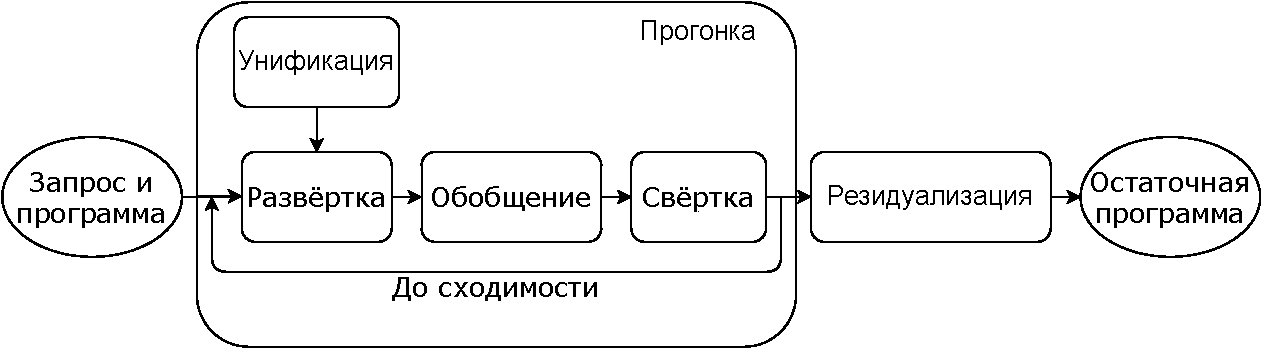
\includegraphics[scale=0.8]{./review/scompflow.pdf}
\caption{Общая схема суперкомпилятора.}
\label{fig:scompScheme}
\end{figure}

% Про "символьное исполнение" https://en.wikipedia.org/wiki/Symbolic_execution
% Сделать ссылку на Ключникова?
%История вычислений представляется в виде {\it графа конфигураций}, где {\it конфигурация}
%описывает состояние вычисления на конкретном шаге. Построение графа происходит на этапе
%{\it прогонки}, во время которого происходит символьное исполнение программы. Потенциально
%такой граф --- который без дополнительных шагов прогонки вырождается в дерево ---
%бесконечный. Для трансформации бесконечного дерева в конечный объект используется {\it cвёртка}
%--- при обработке конфигурации, выражение в которой является {\it переименованием} выражения в одной
%из родительских конфигураций.

История вычислений при суперкомпиляции представляется в виде \emph{графа процессов} --- корневого ориентированного графа,
в котором каждая ветвь --- это отдельный путь вычислений, а каждый узел --- состояние системы или \emph{конфигурация}.
Конфигурация обобщённо описывает множество состояний вычислительной системы или её подсистемы.
% К примеру, конфигурацией можно назвать пару из выражения $1 + x$, которое описывает все возможные суммы с $1$
% свободной переменной $x$, и множество органичений $\{ x \neq 10, x = 1 + x_1 \}$,
% которое сужает множество описываемых состояний до необходимого.
К примеру, конфигурацией можно назвать выражение $1 + x$, в котором параметр $x$ пробегает
все возможные значения своего домена (допустим, множество натуральных чисел) и задаёт
таким образом множество состояний программы\cite{turchinSC}.

Процесс построение графа процессов называется \emph{прогонкой}~\origin{driving}.
Во время прогонки производится шаг символьных вычислений, после которого
в граф процессов добавляются порождённые конфигурации; множество конфигураций
появляется тогда, когда ветвления в программе зависят от свободных переменных.

В процессе прогонки в конфигурациях могут появляться новые свободные переменные,
которые строятся из исходной конфигурации:
если при вычислении выражения его переменная перешла в другую переменную (к примеру, из-за сопоставления с образцом),
то в итоговую конфигурацию будет подставлена новая переменная и связь старой и новой сохранится в
некоторой \emph{подстановке}.
Подстановка --- это отображение из множества переменных в множество возможно замкнутых термов.
Применение подстановки к выражению заменит все вхождения переменных, принадлежащих её домену,
на соответствующие термы. %\todo{Что-нибудь ещё}

Пример графа процессов представлен на рисунке~\ref{fig:pgraphExample}.
\begin{figure}[h!]
\center
\begin{tikzpicture}[->,node distance=3cm, sibling distance=5cm]
                                                            
  \tikzstyle{conf}=[rectangle,draw, rounded corners=.8ex]

  \node[conf] (root) {$(a + b) + c$} ;
  \node[conf] (childLeft) [below left of = root] {$b + c$};
  \node[conf] (childRight)[below right of = root] {$(\text{Succ}(a_1) + b) + c$};
  \path (root) edge node[above left,pos=1] {$\{a \mapsto \text{Zero}\}$} (childLeft)
        (root) edge node[above right,pos=1]{$\{a \mapsto \text{Succ}(a_1)\}$}(childRight);
\end{tikzpicture}

\caption{Пример части графа процессов.}
\label{fig:pgraphExample}
\end{figure}
Здесь при исполнении выражение $(a + b) + c$, где $a, b, c$ -- натуральные числа,
были рассмотрены возможные значения $a$: это либо оно равно нулю (конструктор Zero), либо это некоторое
число $a_1$, которому прибавили единицу (конструктор Succ). Эти два случая могут задают
различные пути исполнения и, соответственно, добавлены в дерево процессов как два различных состояния,
в одно из которых войдёт программа при исполнении.



Потенциально процесс прогонки бесконечный, к примеру, когда происходят рекурсивные вызовы.
Для превращения бесконечого дерева вычисления в конечный объект, по которому множно
восстановить исходное дерево, используется \emph{свёртка.}

Свёртка~\origin{folding}~--- это процесс преобразования дерева процессов в граф, при котором
из вершины $v_c$ добавляется ребро в родительскую вершину $v_p$,
если выражение в конфигурации в $v_c$ и в $v_p$ равны с точностью до переименования.
Пример ситуации для свёртки изображён на рисунке~\ref{fig:pgraphFoldingExample},
на котором свёрточное ребро изображено пунктиром.

\begin{figure}[h!]
\center
\begin{tikzpicture}[->,node distance=2.3cm, sibling distance=5cm]
                                                            
  \tikzstyle{conf}=[rectangle,draw, rounded corners=.8ex]

  \node[conf] (root) {$a + b$} ;
  \node[conf] (childLeft) [below left of = root] {$b$};
  \node[conf] (childRight)[below right of = root] {$(\text{Succ}(a_1) + b)$};
  \node[conf] (childRight2)[below  of = childRight] {$(a_1 + b)$};
  \node (left)[below of = childLeft] {$\cdots$};

  \path (root) edge node[above left,pos=1] {$\{a \mapsto \text{Zero}\}$} (childLeft)
        (root) edge node[above right,pos=1]{$\{a \mapsto \text{Succ}(a_1)\}$}(childRight)
        (childLeft) edge (left)
        (childRight) edge (childRight2)
        (childRight2) edge[bend right=90] (root);
\end{tikzpicture}

\caption{Пример свёртки.}
\label{fig:pgraphFoldingExample}
\end{figure}

Однако существует ситуации, при котором свёртка не приведёт к тому, что граф превратится в
конечный объект. Такое может произойти, к примеру, когда два выражения структурно
схожи, но не существует переименования, уравнивающих их: $a + b$ и $a + a$.

Для решения этой проблемы используется \emph{обобщение}\cite{scGen}. Обобщение --- это процесс
замены одной конфигурации на другую, более абстрактную, описывающую больше состояний
программы. Для обнаружения ``похожей'' конфигурации используется предикат,
традиционно называемый \emph{свистком}: свисток пробегает по всем
родителям текущей конфигурации и определяет, похожа ли конфигурация на кого-то из них.
В случае, когда свисток сигнализирует о найденной схожести, применяется обобщение.
Сам шаг обобщения может произвести действия трёх видов:
\begin{itemize}
\item \emph{обобщение вниз} приводит к тому, что новая конфигурация заменяет текущую в графе процессов;
\item \emph{обобщение вверх} приводит к замене родительской конфигурации на обобщённую;
\item \emph{разделение}~\origin{split} используется для декомпозиции выражении, элементы которого затем
будут обработаны отдельно.
\end{itemize}
Пример обобщения представлен на рисунке~\ref{fig:pgraphGenExample}

\begin{figure}[h!]
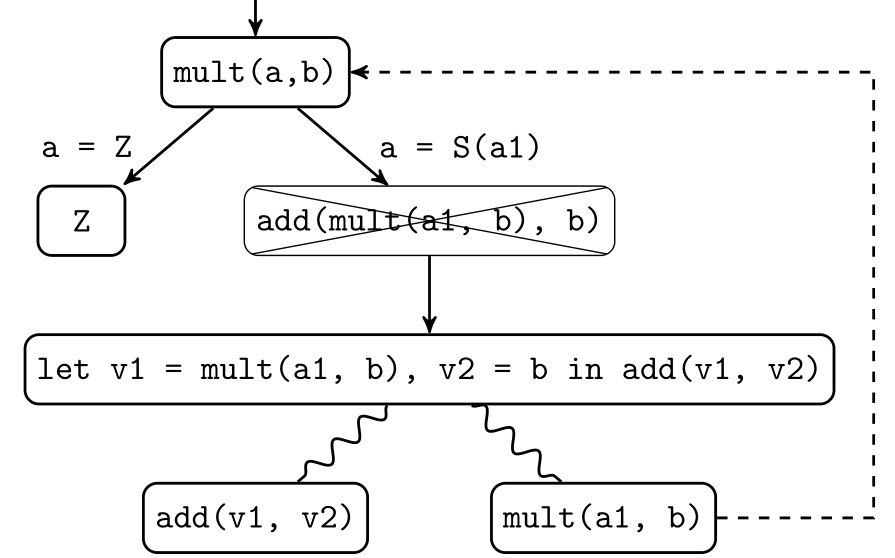
\includegraphics[scale=0.3]{./review/scgenex_temp.png}
\caption{Пример обобщения \todo{свой рисунок}.}
\label{fig:pgraphGenExample}
\end{figure}

Построение программы по графу конфигураций называется \emph{резидуализацией}, а
построенная программа --- \emph{остаточной} \origin{residual}.
Алгоритм выявления остаточной программы основан на обходе дерева, но
в остальном полностью зависит от языка.

% \todo{Написать ещё про СК; продемонстрировать результаты СК; выводы}

Техника суперкомпиляции применяется для функциональных\cite{scHaskell, scPos}
и императивных\cite{scJava} языков. \todo{Кажется, нужны какие-то выводы}



\subsection{Постановка задачи}

Таким образом, целью данной работы является улучшение качества специализации
реляционных программ на miniKanren с использованием методов суперкомпиляции.
Для этого были поставлены следующие задачи:
\begin{itemize}
\item реализовать базовый суперкомпилятор;
\item рассмотреть и реализовать возможные модификации алгоритма суперкомпиляции,
      учитывающие свойства реляционных языков;
\item произвести экспериментальное исследование результата.
\end{itemize}

%\newpage
\section{Специализация miniKanren}

В данной работе для специализации был выбран \ukanren --- минималистичный диалект языка miniKanren\cite{uKanren}.
\ukanren содержит только чистые операторы, что заначительно упрощает процесс специализации.

Абстрактный cинтаксис языка представлен на Рисунке~\ref{fig:syntax}.

\begin{figure}[h!]
\centering
\[\begin{array}{ccll}
  \mathcal{C}   & = & \{C_i\}                                                   &\mbox{конструктор с арностью}\ i \\
  \mathcal{X}   & = & \{ x, y, z, \dots \}                                      &\mbox{переменные} \\
  \mathcal{T}_X & = & X \cup \{C_i (t_1, \dots, t_i) \mid t_j\in\mathcal{T}_X\} &\mbox{термы над множеством переменных $X$} \\
  \mathcal{D}   & = & \mathcal{T}_\emptyset                                     &\mbox{замкнутое выражение}\\
  \mathcal{R}   & = & \{ R_i\}                                                  &\mbox{реляционный символ с арностью}\ i \\[2mm]
  \mathcal{G}   & = & \mathcal{T_X}\equiv\mathcal{T_X}                          &\mbox{унификация} \\
                &   & \mathcal{G}\land\mathcal{G}                               &\mbox{конъюнкция} \\
                &   & \mathcal{G}\lor\mathcal{G}                                &\mbox{дизъюнкция} \\
                &   & \mbox{\lstinline|fresh|}\;\mathcal{X}\;.\;\mathcal{G}     &\mbox{введение свежей переменной} \\
                &   & R_i (t_1,\dots,t_i),\;t_j\in\mathcal{T_X}                 &\mbox{вызов реляционного отношения} \\[2mm]
  \mathcal{S}   & = & \{R_i^j = \lambda\;x_1\dots x_i\,.\, g_j;\}\; g           &\mbox{спецификация программы}
\end{array}\]
\caption{Синтаксис языка \ukanren\cite{semanticMK}.}
\label{fig:syntax}
\end{figure}

\begin{itemize}
\item Унификация двух термов $t_1 \equiv t_2$ порождает подстановку $\theta$, называемую \emph{унификатором},
      такую что её применение к термам уравнивает их: $t_1 \theta = t_2 \theta$.

      Алгоритм унификации языков семейства miniKanren использует проверку вхождения \origin{occurs check},
      что гарантирует корректность получаемых унификаторов, однако довольно сильно замедляет выполнение программ.

\item Конъюнкция двух целей $g_1 \land g_2$ подразумевает одновременное успешное выполнение выражений $g_1$ и $g_2$.
\item Дизъюнкция двух целей $g_1 \lor g_2$ подразумевает, что достаточно, чтобы хотя бы одно из выражений $g_1$ или $g_2$ выполнялось успешно.
      Следует отметить, что при выполнении $g_1$ выражение $g_2$ также будет вычисляться.
\item Введение свежей переменной $\text{fresh}\ x\ .\ g$ в языках miniKanren нужно указывать явно, в отличие, к примеру,
      от Prolog, где это происходит неявно.
\item Вызов реляционного отношения приводит к тому, что переданные в отношение термы
      унифицируются со аргументами отношения и подставляются в тело отношения. 
\end{itemize}

В контексте вычислений важно различие между \emph{синтаксическими} переменными, которые
определяются в тексте программы и обычно представляются строковыми литералами, и
\emph{семантическими} переменными, которые непосредственно используются в процессе вычислений и
представляются целыми числами, с которыми легче работать и генерировать свежие.

\ukanren является ядром языка miniKanren и может быть без труда расширен необходимыми
конструкциями.


\subsection{Библиотека специализации}

Реализация суперкомпилятора для \ukanren строилась на основе проекта по специализации miniKanren с помощью конъюнктивной частичной
дедукции\footnote{\url{https://github.com/kajigor/uKanren_transformations/}} на функциональном языке программирования Haskell.
\todo{...}

%%%%%%%%%%%%%%%%%%%%%%%%%%%%%%%%%%%%%%%%%%%%%%%%%%%%%%%%%
%%%%%%%%%%%%%%%%%%%%%%%%%%%%%%%%%%%%%%%%%%%%%%%%%%%%%%%%%
% Про инстансы и прочее
%%%%%%%%%%%%%%%%%%%%%%%%%%%%%%%%%%%%%%%%%%%%%%%%%%%%%%%%%
%%%%%%%%%%%%%%%%%%%%%%%%%%%%%%%%%%%%%%%%%%%%%%%%%%%%%%%%%
Терм $t_2$ является \emph{экземпляром} \origin{instance} терма $t_1$, если
существует подстановка $\theta$, такая что $t_1 \theta = t_2$.

$t_2$ является \emph{строгим} экземпляром $t_1$, если  $t_2$ является экземпляром $t_1$ и
$t_1$ не является экземпляром $t_2$.
\todo{Почему нам это важно}

%%%%%%%%%%%%%%%%%%%%%%%%%%%%%%%%%%%%%%%%%%%%%%%%%%%%%%%%%
%%%%%%%%%%%%%%%%%%%%%%%%%%%%%%%%%%%%%%%%%%%%%%%%%%%%%%%%%
% Свисток и гомеоморфное вложение
%%%%%%%%%%%%%%%%%%%%%%%%%%%%%%%%%%%%%%%%%%%%%%%%%%%%%%%%%
%%%%%%%%%%%%%%%%%%%%%%%%%%%%%%%%%%%%%%%%%%%%%%%%%%%%%%%%%

В качестве свистка используется отношение \emph{гомеоморфного вложения}.\cite{scGen}
Отношение гомеоморфного вложения $\unlhd$ определено индуктивно:
\begin{itemize}
\item переменные вложены в переменные: $x \embed y$;
\item терм $X$ вложен в конструктор с именем $C$, если он вложен в один из аргументов конструктора:
      $$X \embed C_n(Y_1, \dots, Y_n): \exists i, X \embed Y_i;$$
\item конструкторы с одинаковыми именами состоят в отношении вложения, если в этом отношении
      состоят их аргументы:
      $$C_n(X_1, \dots, X_n) \embed C_n(Y_1, \dots, Y_n): \forall i, X_i \embed Y_i.$$
\end{itemize}

К примеру, выражение $c(b) \embed c(f(b))$, но $f(c(b)) \cancel{\embed} c(f(b))$.

Отношение строгого гомеоморфного вложения $\embed^*$ вводит дополнительное
требование, чтобы терм $X$, состоящий в отношении с $Y$, не был \emph{строгим экземпляром} $Y$. 

Преимущество использования гомеоморфного вложения, в первую очередь, состоит в том,
что для этого отношения доказано, что на бесконечной последовательности выражений $e_0, e_1, \dots, e_n$
обязательно найдутся такие два индекса $i < j$, что $e_i \embed e_j$, вне зависимости
от того, каким образом последовательность выражений была получена~\cite{scPos}.




%%%%%%%%%%%%%%%%%%%%%%%%%%%%%%%%%%%%%%%%%%%%%%%%%%%%%%%%%
%%%%%%%%%%%%%%%%%%%%%%%%%%%%%%%%%%%%%%%%%%%%%%%%%%%%%%%%%
% Обобщение
%%%%%%%%%%%%%%%%%%%%%%%%%%%%%%%%%%%%%%%%%%%%%%%%%%%%%%%%%
%%%%%%%%%%%%%%%%%%%%%%%%%%%%%%%%%%%%%%%%%%%%%%%%%%%%%%%%%

\emph{Наиболее тесное обобщение} \origin{most specific generalization} \todo{вот такое вот оно}.



\subsection{Реализация суперкомпиляции}

%%%%%%%%%%%%%%%%%%%%%%%%%%%%%%%%%%%%%%%%%%%%%%%%%%%%%%%%%%%%%%%%%%%
%%%%%%%%%%%%%%%%%%%%%%%%%%%%%%%%%%%%%%%%%%%%%%%%%%%%%%%%%%%%%%%%%%%
% Описание "графа" процессов
%%%%%%%%%%%%%%%%%%%%%%%%%%%%%%%%%%%%%%%%%%%%%%%%%%%%%%%%%%%%%%%%%%%
%%%%%%%%%%%%%%%%%%%%%%%%%%%%%%%%%%%%%%%%%%%%%%%%%%%%%%%%%%%%%%%%%%%

Представление графа процессов в Haskell затруднено тем, что графовые
структуры данных обычно требуют ссылок на произвольные узлы,
что приводит к появлению перекрёсных ссылок. Прямая реализация этой
идеи сложна в разработке и поддержке и не является идиоматичной.
Использование \emph{IORef}\footnote{https://hackage.haskell.org/package/base-4.11.1.0/docs/Data-IORef.html},
хотя и предоставляет мутабельность, приводит к неоправданному усложнению кода всего проекта,
избавляя код от функциональной чистоты.

Заметим, что графовость этой структуре данных придают \emph{обратные рёбра}
(то есть рёбра от детей к родителям), которые появляются при свёртке, когда ребёнок
является переименованием родителя.
Тогда, если уметь сохранять или восстанавливать информацию об этой связи, то
достаточным будет представить граф в качестве \emph{дерева} процессов.
Древовидные структура однозначно отображается на процесс символьных вычислений,
а также они легко и идиоматично в Haskell.

Структура дерева процессов представлена в виде дерева на рисунке~\ref{fig:ptree}.

\begin{figure}[h!]
\begin{lstlisting}[mathescape,language=Haskell,extendedchars=\true,frame=single,basicstyle=\ttfamily]

type Conf = Conjunction (RelationCall FreeVar)

type Subs = Variable $\mapsto$ Term

data Tree where
  Failure     :: Tree
  Success     :: Subst $\rarrow$ Tree
  Renaming    :: Conf $\rarrow$ Subst $\rarrow$ Tree
  Abstraction :: Conf $\rarrow$ Subst $\rarrow$ List Tree $\rarrow$ Tree
  Generalizer :: Subst $\rarrow$ Tree $\rarrow$ Tree
  Unfolding   :: Conf $\rarrow$ Subst $\rarrow$ List Tree $\rarrow$ Tree
\end{lstlisting}
\caption{Описание дерева процессов.}
\label{fig:ptree}
\end{figure}

Конфигурация \lstinline{Conf} определена как выражение со свободными переменными.
В узле дерева процессов хранится конфигурация, приведённая к форме, содержащей только конъюнкцию вызовов
реляционного отношения. Это сделано из тех соображений, что, во-первых, дизъюнкция представляет
собой ветвление вычислений, посему, соответственно, представляется как ветвление в дереве процессов,
во-вторых, унификации производятся во время символьных вычислений и добавляются в подстановку,
в-третьих, так как введение свежей переменной оказывает влияние лишь на состояние, в котором производятся вычисления,
неосмысленно сохранять его в конфигурации.

Подстановка \lstinline{Subst} соответствует своему математическому определению как отображению из
переменных в термы.
Узлы дерева процессов представляют шаги суперкомпиляции и исходы вычисления выражений:
\begin{itemize}
\item \lstinline{Failure} обозначает неудавшееся вычисления. Такой исход
      случается при появлении противоречивых подстановок;
\item \lstinline{Success}, напротив, обозначает удавшееся вычисление, которое свелось к подстановке \lstinline{Subst};
\item \lstinline{Renaming} обозначает узел, конфигурация которой является переименованием какого-то родительского узла.
\item \lstinline{Abstraction} обознает узел, который может быть обобщён на одного из родителей.
      После обобщения может появится несколько конфигураций, которые являются результатом применения разделения.
      Эти конфигурации добавляются в качестве списка дочерних поддеревьев в текущий узел. 
\item \lstinline{Generalizer} \todo{описать после того, как опишешь обобщение}
\item \lstinline{Unfolding} обознает шаг символьного вычисления, на котором  
\end{itemize}

%%%%%%%%%%%%%%%%%%%%%%%%%%%%%%%%%%%%%%%%%%%%%%%%%%%%%%%%%%%%%%%%%%%
%%%%%%%%%%%%%%%%%%%%%%%%%%%%%%%%%%%%%%%%%%%%%%%%%%%%%%%%%%%%%%%%%%%
% Описание окружения
%%%%%%%%%%%%%%%%%%%%%%%%%%%%%%%%%%%%%%%%%%%%%%%%%%%%%%%%%%%%%%%%%%%
%%%%%%%%%%%%%%%%%%%%%%%%%%%%%%%%%%%%%%%%%%%%%%%%%%%%%%%%%%%%%%%%%%%

\emph{Окружение} для суперкомпиляции должно сохранять следующие объекты:
\begin{itemize}
\item подстановку, в которой содержатся все накопленные непротиворечивые унификации,
      необходимую в процессе прогонки для проверки новых унификаций;
\item первую свободную семантическую переменную, необходимую для генерации свежих переменных,
      к примеру, при абстракции;
\item определение программы, необходимое для замены вызова на своё тело.
\end{itemize}

\todo{Что-то ещё об этом нужно написать!}

%%%%%%%%%%%%%%%%%%%%%%%%%%%%%%%%%%%%%%%%%%%%%%%%%%%%%%%%%%%%%%%%%%%
%%%%%%%%%%%%%%%%%%%%%%%%%%%%%%%%%%%%%%%%%%%%%%%%%%%%%%%%%%%%%%%%%%%
% Описание шага unfolding'а
%%%%%%%%%%%%%%%%%%%%%%%%%%%%%%%%%%%%%%%%%%%%%%%%%%%%%%%%%%%%%%%%%%%
%%%%%%%%%%%%%%%%%%%%%%%%%%%%%%%%%%%%%%%%%%%%%%%%%%%%%%%%%%%%%%%%%%%

Шаг символьного вычисления по данной конфигурации $C$ порождает
множество конфигурации $\{ C_1, \dots, C_n \}$, описывающих состояния в которое может перейти
процесс реального исполнения программы. Классически, шаг символьного
вычисления соответствует семантике языка, который суперкомпилируется,
и для \ukanren существует сертифицированная семантика\cite{semanticMK},
однако описание шага символьного вычисления \ukanren для суперкомпиляции 
усложнено тем, что реляционные языки не исполняются привычным образом,
как, к примеру, функциональные программы, и \emph{поиск}, вшитый в семантику,
не ложится на суперкомпиляцию.

Тогда порождённую конфигурацию можно рассматривать не как непосредственный
шаг вычисления, но как возможное состояние, в которое может перейти программа.
Такое состояние появляется путём раскрытия тела одного или нескольких
конъюнктов конфигурации.

К примеру, рассмотрим часть программы на \ukanren на рисунке~\ref{fig:unfoldEx}, в котором
определены какие-то отношения \lstinline{f} и \lstinline{g}.
\begin{figure}[h!]
\begin{lstlisting}
f(a) = f'(a)$\lor$f''(a)
g(a, b) = g'(a)$\land$g''(b)
\end{lstlisting}
\caption{Пример отношений для демонстрации шага символьных вычислений}
\label{fig:unfoldEx}
\end{figure}

Допустим, на шаге суперкомпиляции алгоритм обрабаывает конфигурацию
\lstinline{f($\text{v}_\text{1}$)$\land$g($\text{v}_\text{1}$, $\text{v}_\text{2}$)}
хотим сделать шаг символьного вычисления. Рассмотрим несколько способов породить новые конфигурации.
\begin{itemize}
\item Если раскроется определение \lstinline{f}, то будут получены новые конфигурации 
      \lstinline{f'($\text{v}_\text{1}$)$\land$g($\text{v}_\text{1}$, $\text{v}_\text{2}$)} и
      \lstinline{f''($\text{v}_\text{1}$)$\land$g($\text{v}_\text{1}$, $\text{v}_\text{2}$)}.
\item Если раскроется определение \lstinline{g}, то будет получена новая конфигурация 
      \lstinline{f($\text{v}_\text{1}$)$\land$g'($\text{v}_\text{1}$)$\land$g''($\text{v}_\text{2}$)}.
\item Если раскроются оба определения \lstinline{f} и \lstinline{g}, то будут получены новые конфигурации 
      \lstinline{f'($\text{v}_\text{1}$)$\land$g($\text{v}_\text{1}$)$\land$g''($\text{v}_\text{2}$)} и
      \lstinline{f''($\text{v}_\text{1}$)$\land$g($\text{v}_\text{1}$)$\land$g''($\text{v}_\text{2}$)}.
\end{itemize}

Последний набор конфигураций --- это полный набор состояний, в которые процесс вычислений может
прийти. В первых двух наборах, можно отметить, порождённые конфигурации не исключают
возможные состояния процессов, отображённые в последнем наборе, они могут появится на последующих шагах вычисления,
если перед этим ветвь исполнения не будет остановлена из-за противоречивой подстановки.

Таким образом, какой-бы способ развёртывания определений не был бы выбран, он не будет
исключать состояния, в которые процесс вычисления теоретически может прийти, но выбор
разных стратегий развёртывания может систематически приводить к разным деревьям процессов,
а следовательно, приводить к различным эффектам специализации.

Базовой стратегией порождения новых конфигураций выбрана \emph{полная стратегия развёртывания},
пример которой был показан выше, при которой мы заменяем определния всех реляционных вызовов
конфигурации.

%%%%%%%%%%%%%%%%%%%%%%%%%%%%%%%%%%%%%%%%%%%%%%%%%%%%%%%%%%%%%%%%%%%
%%%%%%%%%%%%%%%%%%%%%%%%%%%%%%%%%%%%%%%%%%%%%%%%%%%%%%%%%%%%%%%%%%%
% Описание общего алгоритма суперкомпиляции
%%%%%%%%%%%%%%%%%%%%%%%%%%%%%%%%%%%%%%%%%%%%%%%%%%%%%%%%%%%%%%%%%%%
%%%%%%%%%%%%%%%%%%%%%%%%%%%%%%%%%%%%%%%%%%%%%%%%%%%%%%%%%%%%%%%%%%%

\subsubsection{Обобщённый алгоритм суперкомпиляции}

Обобщённый алгоритм суперкомпиляции представлен на рисунке~\ref{fig:scalgogen}.
\todo{Подробнее:)}

\begin{figure}[h!]
\begin{lstlisting}[mathescape,language=Haskell,extendedchars=\true,frame=single,basicstyle=\ttfamily]
drive(env, tree, expression):
  if expression is empty
  then add(env, tree, success node)
  else if $\exists \text{parent}:$ expression is renaming of parent
  then add(env, tree, renaming node)
  $\text{\color{red}TODO: Ввести нотацию для } \embed^+$
  else if $\exists$ parent: parent $\embed^+$ expression
  then
     node $\larrow$ abstractUp(expression, parent)
     addUp(env, tree, parent, node)
  else else if $\exists$ parent: parent $\embed^*$ expression
  then
    add(abstraction, node)
    children $\larrow$ abstract(expression, parent)
    $\forall \text{child} \in \text{children}:$
      drive(tree, child)
  else
    add(unfolding node)
    children $\larrow$ unfold(expression)
    $\forall \text{child} \in \text{children}:$
      drive(tree, child)
\end{lstlisting}
\caption{Обобщённый алгоритм суперкомпиляции}
\label{fig:scalgogen}
\end{figure}


%%%%%%%%%%%%%%%%%%%%%%%%%%%%%%%%%%%%%%%%%%%%%%%%%%%%%%%%%%%%%%%%%%%
%%%%%%%%%%%%%%%%%%%%%%%%%%%%%%%%%%%%%%%%%%%%%%%%%%%%%%%%%%%%%%%%%%%
% Описание конкретного алгоритма суперкомпиляции
%%%%%%%%%%%%%%%%%%%%%%%%%%%%%%%%%%%%%%%%%%%%%%%%%%%%%%%%%%%%%%%%%%%
%%%%%%%%%%%%%%%%%%%%%%%%%%%%%%%%%%%%%%%%%%%%%%%%%%%%%%%%%%%%%%%%%%%
\subsubsection{Конкретный алгоритм суперкомпиляции}

Наличие операции обобщения вверх предполагает, что необходимо умение передвигаться по дереву вверх и изменять его. 
Реализация в Haskell этой идеи --- задача крайне нетривиальная. Возможно представлять
деревья в мутабельных массивах, однако при обобщении необходимо удалять целые поддеревья,
что при таком подходе сложная операция.

Классическим способом решения этой проблемы являются \emph{зипперы}\cite{zipper}.
Эта идиома предлагает рассматривать структуру данных как пару из элемента,
на котором установлен фокус, и контекста, который представляется как структура данных
с ``дыркой'', в котором сфокусированный элемент должен находиться.

К примеру, зиппер для списка \lstinline{[1, 2, 3, 4]} при фокусе на 3 представляется
таким образом: \lstinline{(3, ([2, 1, 0], [4, 5, 6]))}.
Тогда перефокусировка вправо или влево на один элемент происходит за константу,
как и замена элемента, для которой достаточно заменить первую компоненту пары.
В то время как, в силу того, что операция взятия элемента в связном списке по индексу
происходит за линейное время от длины списка, взятие элемента слева от 3 также
будет происходить за линейное время, как и, соответственно, модификация списка.

Для деревьев с произвольным количеством детей зиппер может выглядеть
как пара из текущего узла и списка родителей, отсортированного в порядке
близости к узлу (рисунок~\ref{fig:zipper}). 
\begin{figure}[h!]
\begin{lstlisting}[mathescape,language=Haskell,extendedchars=\true,frame=single,basicstyle=\ttfamily]
data Parent = Parent { children :: ListZipper Node }
type TreeZipper = (Node, List Parent)
\end{lstlisting}
\caption{Пример структуры зиппера для деревьев}
\label{fig:zipper}
\end{figure}

Родительский (структура \lstinline{Parent}) cписок детей представлен в виде зиппера (поле \lstinline{children})
для списка, в котором происходит фокус: у непосредственного родителя --- на элемент в фокусе, а у остальных
родителей --- на предыдущего в порядке сортировки.\todo{more?}

При представлении дерева процессов в идиоме зипперов основа алгоритма суперкомпиляции
принимает форму описания действий при смене состояния зиппера.
\todo{TODO}

\subsubsection{Модификации базового алгоритма суперкомпиляции}

\paragraph{Поиск узлов для переименования среди всех вычисленных поддеревьев}\ \\
В базовом алгоритме суперкомпиляции поиск узлов на которые происходят переименования происходит
среди родителей. Это напрямую соотносится с понятием символьных вычислений: по достижении
узла, которое является переименованием уже встреченного, вычисление переходит на родительский узел.
Однако довольно части встречается, что в разных поддеревьях дерева процессов стречаются одинаковые
конфигурации, поддеревья которых оказываются полностью идентичными. В таком случае, кажется
очевидной оптмизация, при которой мы запоминаем вычисленные поддеревья и в случае,
когда мы встречаем схожу конфигурацию, не вычисляем поддерево заново, добавляя ссылку на него.
\todo{Показать, почему это ничего не сломает}

\paragraph{Стратегии развёртывания реляционных вызовов}\ \\
Как уже говорилось, разные стратегии развёртывания реляционных вызовов могут привести к разным
эффектам специализации. К примеру, полная стратегия развёртывания, которая была принята за базовую,
приводит к \emph{таплингу} \origin{tupling}\cite{tupling} --- оптмизации, при которой
множество проходов по одной структуре данных заменяется на один проход.

% Может, показать, что оно круто всё строит?

Основной недостаток базового подхода в том, что он для получения всех возможных состояний
производит декартово производение тел вызовов в конъюнкциях, что приводит
к сильному разрастанию дерева процессов и, как следствия, сильно требователен к вычислительным ресурсам.
Вследствие чего реализация новых стратегий развёртывания производится не только в исследовательских,
но и прикладных целях.

Для лёгкой подмены стратегий суперкомпиляции был разработан специальный интерфейс \lstinline{UnfoldableGoal}
(рисунок~\ref{fig:unfoldable}).
\begin{figure}[h!]
\begin{lstlisting}
class Unfoldable a where
   initialize :: Conf $\rarrow$ a
   get        :: a $\rarrow$ Conf
   unfoldStep :: a $\rarrow$ Env $\rarrow$ List (Env, a)
\end{lstlisting}
\caption{Интерфейс для различных стратегий развёртывания.}
\label{fig:unfoldable}
\end{figure}

Предоставляемые интерфейсом функции используются в алгоритме суперкомпиляции следующим образом:
\begin{itemize}
\item \lstinline{initialize} оборачивает конфигурацию в структуру, в которой может содержаться
      вспомогательная информация для процесса развёртывания;
\item \lstinline{get} позволяет получить конфигурацию для применения её к операциям, не зависящим
      от стратегий;
\item \lstinline{unfoldStep} непосредственно проводит шаг вычисления на основе текущей конфигурации
      и её окружения, порождая новые конфигурации с соответствующими им состояниями.
\end{itemize}

В работе рассмотрен и реализован ряд стратегий, описанные ниже.

\begin{itemize}
\item {\bf Последовательная стратегия развёртывания}, при которой отслеживается,
      какой вызов был раскрыт на предыдущем шаге, чтобы на текущем
      раскрыть следующий за ним.\todo{todo}
\item {\bf Нерекурсивная стратегия развёртывания}, при которой в первую очередь
      раскрывается нерекурсивный вызов в конфигурации. Нерекурсивность определяется
      лишь тем, содержит ли определение реляционный вызов самого себя. Более сложный
      анализ структуры функций не мог бы быть использован в силу того, что тогда
      было бы необходимо реализовать класс алгоритмов анализа, что совершенно отдельная задача.

      Ожидается, что при нерекурсивной стратегии развёртывания из конфигураций
      будут как можно быстрее появляться выражения, которые могут быть сокращены
      или вовсе удалены из-за унификации (к примеру, отношения, кодирующие
      таблицы истинности, такие как \rel{and}) или привести к скорой свёрте.
      \todo{todo}.

\item {\bf Стратегия развёртывания вызовов с минимальным количеством ветвлений},
      при которой на каждом шаге вычисления будет появляться минимально возможное количество
      конфигураций, что приведёт к минимальной ветвистости дерева.
\end{itemize}

% \subparagraph{Смешанная стратегия развёртывания}
% \todo{Ещё нужно бы проработать}

\paragraph{Частичный или полный отказ от обобщения вверх}\ \\
Обобщение вверх приводит к тому, что происходит замена целого поддерева процессов
предка, на которого обобщается конфигурация. Иногда это может приводить к тому, что
теряются аргументы частично известного входа. К примеру, на рисунке~\ref{fig:genup}
представлено дерево процессов, при котором происходит обобщение вверх.
\begin{figure}[h!]
\center
\begin{tikzpicture}[->,node distance=2cm, sibling distance=5cm]
                                                            
  \tikzstyle{conf}=[rectangle,draw, rounded corners=.8ex]

  \node[conf] (root) {\rel{reverse}($a$, $a$)} ;
  \node[conf] (gen) [below of = root] {Generalizer: $\{ v_1 \mapsto a, v_2 \mapsto a \}$};
  \node[conf] (node) [below of = gen] {\rel{reverse}($v_1$, $v_2$)};
  \node (rest)[below of = node] {$\cdots$};
   \path (root) edge (gen)
         (gen) edge (node)
         (node) edge (rest);
  % \path (root) edge node[above left,pos=1] {$\{a \mapsto \text{Zero}\}$} (childLeft)
  %       (root) edge node[above right,pos=1]{$\{a \mapsto \text{Succ}(a_1)\}$}(childRight)
  %       (childLeft) edge (left)
  %       (childRight) edge (childRight2)
  %       (childRight2) edge[bend right=90] (root);
\end{tikzpicture}
\caption{Демонстрация потери информации при обобщении вверх.}
\label{fig:genup}
\end{figure}
\todo{пояснения к примеру}

В случае же, когда обощение происходит на сам корень дерева, теряется эффект протягивания
констант.


%\newpage
\section{Экспериментальное исследование}
\label{sec:testing}

\subsection{Тестовое окружение}

В качестве основной конкретной реализации \ukanren для тестирования
использовался OCanren\footnote{Проект OCanren: \url{https://github.com/JetBrains-Research/OCanren}, дата последнего посещения: 15.05.2020}\cite{ocanren},
реализованный на OCaml\cite{ocanren}.
%Для некоторых тестов для использовался faster-miniKanren\footnote{\url{https://github.com/miniKanren/faster-miniKanren}},
%версия miniKanren, реализованная на Scheme.

Тесты запускались на ноутбуке со следующими характеристиками: Intel Core i5-6200U CPU, 2.30GHz, DDR4, 12GiB.

Для тестирования суперкомпилятора и его модификаций использовался следующий алгоритм.
\begin{enumerate}
\item Подготавливается программа, реализованная на внутреннем представлении $\mu$Kanren.
\item Программа и запрос, на который будет происходить специализация, подаются на вход суперкомпилятору.
\item По дереву процессов, порождённому суперкомпилятором, строится остаточная программа.
\item Остаточная программа транслируется в OCanren и
      запускается в заранее подготовленном окружении с тестовыми запросами.
\end{enumerate}


Реализованный суперкомпилятор сравнивался с реализацией \forcpd для $\mu$Kanren\footnote{Проект: \url{https://github.com/kajigor/uKanren_transformations}, дата последнего посещения: 15.05.2020},
а также c реализацией \forcpd для Prolog --- системой ECCE\footnote{Проект ECCE: \url{https://github.com/leuschel/ecce}, дата последнего посещения: 15.05.2020}.
Другие специализаторы не рассматриваются, так как согласно работе~\cite{controlPoly}, специализация с
помощью \forcpd в ECCE показывает лучшие результаты.

Для использования последнего требовалось оттранслировать программу на \ukanren в Prolog, специализировать
её на запрос, далее оттранслировать результирующую программу в OCanren.
Это допустимо сделать в силу того, что между \ukanren и чистым подмножеством Prolog есть
взаимно однозначное синтаксическое соответствие. 
Все необходимые средства для этого также предоставлялись указанной библиотекой специализации.


\subsubsection{Набор тестов}

Был выбран следующий набор тестов для тестирования и анализа суперкомпилятора и его модификаций.
\begin{itemize}
 \item Программа \lstinline{doubleAppend(xs, ys, zs, rs)}, которая
       производит конкатенацию трёх списков. Она классически используется
       для проверки эффекта дефорестации в специализированной программе.
       Специализация происходила на запрос \lstinline{doubleAppend} со свободными переменными.
 \item Программа \lstinline{maxLength(xs, max, len)}, которая находит в списке
       максимальный элемент и длину списка. Она классически используется
       для проверки эффекта таплинга в специализированной программе. 
       Специализация происходила на запрос \lstinline{maxLength} со свободными переменными.
 \item Программа сортировки \lstinline{sort(list, result)}. Выбрана в силу показательности
       результатов.
       Специализация происходила на запрос \lstinline{sort} со свободными переменными.
%     Запросы:
%     \begin{itemize}
%     \item оптимизация сортировки: \rel{sort}(xs, ys);
%     \item генерация отсортированных последовательностей: \rel{sort}(xs, xs).
%     \end{itemize}
 \item Отношение, проверяющее принадлежность пути графу \\
       \lstinline{isPath(path, graph, result)}.
       Специализация происходила на запрос \lstinline{isPath(path, graph, True)}.
       Запросы к программе для тестирования:
       \begin{itemize}
       \item поиск пути заданного размера в случайном графе: \\
       \lstinline{isPath(path, graph, True)$\land$length(path, N)};
       \item поиск фиксированного количества путей, принадлежащих данному графу.
       %\\ $\text{isPath}^o_s$(p, g)$\land$\rel{length}(p, N).
       \end{itemize}

	   В приложении А на рисунке~\ref{fig:graphGen} представлен код, который
	   был использован для генерации графов. Функции на вход
	   подаётся количество вершин, количество рёбер и зерно для генератора случайных чисел.
	   В тестах приводятся три графа на 20 вершинах с 50 рёбрами
	   с зёрнами: граф 1 --- 42, граф 2 --- 34, граф 3 --- 106.

 \item Интерпретатор формул логики высказываний \\ \lstinline{logint(formula, subst, result)}.
       Интерпретатор специализируется на то, чтобы всегда генерировать выполнимые формулы
       \lstinline{logint(formula, subst, True)}.
%      Запросы:
%     \begin{itemize}
%     \item поиск $n$ решений заданной формулы;
%     \item генерация $n$ формул с подстановке размера $n$.
%     \end{itemize}
 \item Интерпретатор лямбда-исчисления \lstinline{lam(expr, result)}.
       Интерпретатор специализируется на выражение \lstinline{lam(expr, result)}
       и используется для генерации $n$ выражений в нормальной форме \lstinline{lam(expr, expr)};
 	%\item генерация $n$ выражений, редуцирующихся к заданному выражению \lstinline{lam(expr, E)}.
 \item Проверка типов в просто типизировнном лямбда-исчислении \lstinline{infer(typ, expr)}.
%   \begin{itemize}
% 	\item Поиск $n$ обителей заданного типа.
% 	\item
     Отношение использовалось для генерация выражений, соответствующих заданной спецификации типа и выржения.
     Специализируется выражение:\\
 	 %\rel{infer}(type, expr) $\land$ type $\equiv$ TYPE\_SPEC $\land$ expr $\equiv$ EXPR\_SPEC.
 	 \lstinline{infer(typ, expr)$\land$typ $\equiv$ TYPE_SPEC$\land$expr $\equiv$ EXPR_SPEC}
 %  \end{itemize}
% \item Интерпретатор простого подмножества Scheme.
%    \begin{itemize}
%    \item \todo{Интересный тест!}
%    \end{itemize}
\end{itemize}

% Все вышеперечисленные программы были применены к реализованным суперкомпиляторами,
Ко всем вышеперечисленным программам были применены суперкомпиляторы, 
и результаты выполнения остаточных программ были проверены на адекватность и соответствие задачам исходных программ.
Проводилось 10 измерений, пока которым выводились средние значения.
Следует отметить, что задачи доказательства сохранения семантики суперкомпилятором на стояло. 

\subsection{Пример работы базового суперкомпилятора \ukanren}
% Для начала разберём, как базовый суперкомпилятор ведёт себя на
% базовом наборе программ, результат которых несложно проанализировать.

% \begin{itemize}
% \item Классическая программа \lstinline{doubleAppend}~\cite{cpd}, которая используется для
%       проверки наличия эффекта дефорестации (\todo{В приложении}).
% %\item Другая классическая программа \lstinline{maxLength}~\cite{cpd}, которая
% %      используется для проверки наличия эффекта таплинга.
% \end{itemize}

Разберём на примере результат работы базового суперкомпилятора.

Классическая программа для тестирования эффектов специализации ---
\lstinline{doubleAppend}, представленная на рисунке~\ref{fig:dappCode},
в которой происходит конкатенация списков трёх списков.

\begin{figure}[h!]
\begin{lstlisting}
doubleAppend a b c d =
  fresh (t)
   (append a b t $\land$ append t c d)
append y4 y5 y6 =
  (y4 $\equiv$ [] $\land$ y6 $\equiv$ y5) $\lor$
  fresh (ty t h)
   (y4 $\equiv$ h :: t $\land$
    y6 $\equiv$ h :: ty $\land$
    append t y5 ty)
\end{lstlisting}
\caption{Программа для тестирования \lstinline{doubleAppend}}
\label{fig:dappCode}
\end{figure}

Во многих бенчмарках~\cite{cpdPract, controlPoly} это программа используется
для проверки эффекта дефорестации.

Рассмотрим дерево процессов на рисунке~\ref{fig:dappTree}
(для компактности \lstinline{append} сокращён до \lstinline{app}),
которое порождается применением базового
суперкомпилятора к программе \lstinline{doubleAppend}, причём в
качестве аргументов --- простые свободные переменные, из-за чего
просто оптимизируется сама структура программы.

\begin{figure}[h!]
\center
\begin{tikzpicture}[->,node distance=3cm, sibling distance=6.2cm, level distance=2cm]
  \tikzstyle{conf}=[rectangle,draw, rounded corners=.8ex,align=center]
  \node[conf] (root)   at (0, 0)     {{\it Unfolding} \\ \lstinline{doubleAppend(a, b, c, abc)}};
  \node[conf] (appapp) at (0, -2)    {{\it Unfolding} \\ \lstinline{app(a, b, $\text{v}_0$)$\land$app($\text{v}_0$, c, abc)}};
  \node[conf] (app1)   at (-0.3, -6) {{\it Unfolding} \\ \lstinline{app($\text{v}_1$, c, $\text{v}_2$)} \\ $\{$ a $\mapsto$ [], b $\mapsto$ $\text{v}_0$, \\ $\text{v}_0 \mapsto \_ : \text{v}_1$, \\ $\ \ $ abc $\mapsto \_ : \text{v}_2$ $\}$};
  \node[conf] (app2)   at (7, -5.39) {{\it Renaming} \\ \lstinline{app($\text{v}_5$, b, $\text{v}_6$)$\land$app($\text{v}_6$, c, $\text{v}_7$)} \\ $\{$ a $\mapsto \text{h} : \text{v}_5$  $\text{v}_0 \mapsto \text{h} : \text{v}_6 $  abc $\mapsto \text{h} : \text{v}_7$  $\}$};
  \node[conf] (appS)   at (-4,-6)    {{\it Success} \\ $\{$ a $\mapsto$ [], \\ \ \ b $\mapsto$ [],\\ \ \ $\text{v}_0 \mapsto$ [], \\ \ \ c $\mapsto$ abc $\}$};
  \node[conf] (app11)  at (2,  -10)  {{\it Renaming} \\ \lstinline{app($\text{v}_3$, c, $\text{v}_4$)} \\ $\{\text{v}_1 \mapsto \_ : \text{v}_3 $ \\ $\ \ \ \ \text{v}_2 \mapsto \_ : \text{v}_4 $  $\}$};
  \node[conf] (app1S)  at (-2, -9.7) {{\it Success} \\ $\{ \text{v}_1 \mapsto [],$ \\ $\ \ c \ \mapsto \text{v}_2 \}$};
  \draw[-latex] (root) -- (appapp);
  \draw[-latex] (appapp) -- (appS.north);
  \draw[-latex] (appapp) -- (app1);
  \draw[-latex] (appapp) -- (app2);
  \draw[-latex] (app1) -- (app1S);
  \draw[-latex] (app1) -- (app11);
  \draw[-latex,dashed] (app2) edge [bend right] (root);
  \draw[-latex,dashed] (app11) edge [bend right] (app1);
\end{tikzpicture}
\caption{Дерево процессов для программы \lstinline{doubleAppend}}
\label{fig:dappTree}
\end{figure}

В приведённом дереве первым этапом происходит замена определения \lstinline{doubleAppend}
на его тело. Так как в определении нет дизъюнкий, получаем всего одну конфигурацию,
в которой операцией \lstinline{fresh} добавляется новая семантическая переменная $\texttt{v}_0$.
Далее происходит обработка конфигурации с более чем одним конъюнктом. Так как используется
полная стратегия развёртывания, каждая из конъюнкий раскрывается по определению и
рассматривается их дизъюнктивная нормальная форма, в которой всего четыре дизъюнкта,
один из которых не унифицируется, поэтому всего появляется только три конфигурации.
Эти конфигурации рассматривают несколько возможных значений переменных:
\begin{enumerate}
\item когда \lstinline{a} и \lstinline{b} пустые списки, то результатом конкатенации
является \lstinline{c};
\item если же \lstinline{b} не пуст, тогда результат --- это конкатенация списков \lstinline{b} и \lstinline{c}.
      Отношение конкатенации двух списков также специализируется под задачу.
      В результате этой специализации порождается исходное отношение, поскольку
      никакой новой информации не было выявлено и исходная программа уже была оптимальна;
\item в третьем же случае выводится, что результат конкатенации трёх списков
      \lstinline{a}, \lstinline{b} и \lstinline{c} --- это конкатенация
      списков $\texttt{v}_5$, \lstinline{b} и \lstinline{c}, где $\texttt{v}_5$
      является хвостом списка, а в голову которой добавили голову \lstinline{a}.
\end{enumerate}

По данному дереву порождается остаточная программа, изображённая на рисунке~\ref{fig:dappCodeOpt}.
\begin{figure}[h!]
\begin{lstlisting}
doubleAppendo a b c d =
  fresh (x4) (app3 a b x4 c d)
app3 a b t c d =
   fresh (x7 x6 x5 x10 x9 x8)
     (a $\equiv$ [] $\land$ b $\equiv$ t $\land$
       (t $\equiv$ [] $\land$ c $\equiv$ d $\lor$
       (t $\equiv$ x8 :: x9) $\land$
        d $\equiv$ x8 :: x10 $\land$
        app2 x9 c x10
     ) $\lor$
     (a $\equiv$ x5 :: x6 $\land$
      t $\equiv$ x5 :: x7 $\land$
      d $\equiv$ x5 :: x10 $\land$
      app3 x6 b x7 c x10) ) 
app2 a b c =
  fresh (x13 x12 x11)
   (a $\equiv$ [] $\land$ b $\equiv$ c $\lor$
   (a $\equiv$ x11 :: x12 $\land$
    c $\equiv$ x11 :: x13 $\land$
    app x12 b x13))
\end{lstlisting}
\caption{Суперкомпилированная программа \lstinline{doubleAppend}}
\label{fig:dappCodeOpt}
\end{figure}

В итоге, наблюдается, как двупроходный алгоритм становится однопроходным.


\subsection{Сравнение вариаций суперкомпилятора \ukanren}

В таблицах используются условные обозначения для стратегий развёртывания:
\begin{itemize}
\item {\it Full} и {\it Full-non-rec} обозначают полную стратегию и полную стратегию развёртывания с приоритетом на нерекурсивные вызовы соответственно;
\item {\it Seq} обозначает последовательную стратегию развёртывания;
\item {\it Non-rec} и {\it Rec} обозначают нерекурсивную и рекурсивную стратегии соответственно;
\item {\it Min} и {\it Max} обозначают минимальную и максимальную стратегии соответственно;
\item {\it First} обозначает стратегию, при которой всегда развёртывается первый конъюнкт.
\end{itemize}

А также для суперкомпиляторов:
\begin{itemize}
\item {\it Б.С.} обозначает базовый суперкомпилятор с обобщением вниз на предков;
\item {\it М.1 } обозначает модификацию, при которой происходит запрет на обобщение сразу после обобщения;
\item {\it M.2 } обозначает модификацию, при которой обобщение происходит на все ранее вычисленные вершины;
\item {\it M.3 } обозначает модификацию, при которой происходит обобщение вверх на родительские вершины;
\item {\it M.4 } обозначает модификацию, при которой происходит обобщение вверх на родительские вершины, кроме корневой.
\item {\it M.5 } обозначает модификацию, при которой происходит обобщение вверх на родительские вершины, а также запрет обобщения после обобщения.
\end{itemize}


В таблице~\ref{fig:dappTest} представлены результаты сравнения модификаций
с базовым суперкомпилятором при разных стратегиях развёртывания.
При полных стратегиях для \lstinline{doubleAppend} возникает эффект дефорестации.
В остальных стратегиях этого не происходит, из-за чего исполнения по
крайней мере в два раза хуже. Из-за того, что программа довольно небольшая,
модификации алгоритма суперкомпиляции хотя не и оказывают влияния, результат не ухудшают.

\begin{table}[h!]
\center
\begin{tabular}{|l|c|c|c|c|c|c|}
\hline
                   &{\it Б.С.}&{\it М.1}&{\it М.2}&{\it М.3}&{\it M.4} & {\it M.5} \\ \hline
%Original: 0.010374
%ECCE: 0.004058
%CPD: 0.012664
{\it Full        }& {\bf 0.0049}  & 0.0055       & 0.0056       & {\bf 0.0050} & {\bf 0.0048} & 0.0053\\ \hline
{\it Full-non-rec}& 0.0053        & {\bf 0.0048} & {\bf 0.0049} & {\bf 0.0050} & {\bf 0.0037} & {\bf 0.0039} \\ \hline
{\it Seq         }& 0.0098        & 0.0119       & 0.0099       & 0.0127       & 0.0097       & 0.0102 \\ \hline
{\it Non-rec     }& 0.0100        & 0.0122       & 0.0099       & 0.0099       & 0.0097       & 0.0098 \\ \hline
{\it Rec         }& 0.0094        & 0.0133       & 0.0103       & 0.0098       & 0.0097       & 0.0100 \\ \hline
{\it Min         }& 0.0096        & 0.0122       & 0.0100       & 0.0093       & 0.0094       & 0.0099 \\ \hline
{\it Max         }& 0.0096        & 0.0096       & 0.0092       & 0.0101       & 0.0119       & 0.0091 \\ \hline
{\it First       }& 0.0120        & 0.0094       & 0.0094       & 0.0099       & 0.0093       & 0.0093 \\ \hline

\end{tabular}
\caption{Результат для \lstinline{doubleAppendo} c конкатенацией трёх списков длины 120, секунды}
\label{fig:dappTest}
\end{table}

В таблице~\ref{fig:maxlenTest} указаны результаты выполнения для
программы \lstinline{maxLength} на списке \lstinline{[1..200]}.

\begin{table}[h!]
\center
\begin{tabular}{|l|c|c|c|c|c|c|}
\hline
                  &{\it Б.С.}   &{\it М.1}      &{\it М.2}      &{\it М.3}&{\it M.4} & {\it M.5}\\ \hline
%Orig: 0.270905
%ECCE: 0.230436
%CPD: 0.653551
{\it Full        } & 0.623        & 0.638       & {\bf 0.250}  & {\bf 0.250} & {\bf 0.251} & 0.293 \\ \hline
{\it Full-non-rec} & 0.633        & 0.611       & 0.602        & 0.256       & 0.258 & 0.298 \\ \hline
{\it Seq         } & 0.285        & 0.290       & 0.289        & 0.289       & 0.287 & 0.286 \\ \hline
{\it Non-rec     } & 0.284        & 0.289       & 0.285        & 0.285       & 0.287 & 0.287 \\ \hline
{\it Rec         } & 0.856        & 0.893       & 0.560        & 0.577       & 0.569 & 0.888 \\ \hline
{\it Min         } & 0.317        & {\bf 0.280} & 0.303        & 0.284       & 0.279 & {\bf 0.280} \\ \hline
{\it Max         } & {\bf 0.279}  & 0.287       & 0.279        & 0.278       & 0.284 & 0.281 \\ \hline
{\it First       } & 0.864        & 0.858       & 0.564        & 0.963       & 0.949 & 0.565 \\ \hline


\end{tabular}
\caption{Запуск для \lstinline{maxLength} на списке \lstinline{[1..200]}, секунды}
\label{fig:maxlenTest}
\end{table}

Модификация алгоритма {\it M.2-M.4} на стратегии {\it Full} породили программы
с эффектов таплинга, при котором максимальный элемент и длина списка высчитывались
за один проход. Интересное наблюдение состоит в том, что в других случаях, к примеру,
при применении стратегии {\it Seq}, таплинга не происходит, но сама программа
исполняется не существенно медленнее.

В таблице~\ref{fig:sortTest} указаны результаты тестирования для
программы \lstinline{sort} при сортировки списков случайного содержания (числа от 0 до 50)
длины 50.

\begin{table}[h!]

\center
\begin{tabular}{|l|c|c|c|c|c|c|}
\hline
                  &{\it Б.С.}&{\it М.1}&{\it М.2}&{\it М.3}&{\it M.4}&{\it M.5}\\ \hline
{\it Full        } & {\bf 0.239} & 0.252       & {\bf 0.238} & {\bf 0.232} & {\bf 0.239} & 0.244 \\ \hline
{\it Full-non-rec} & 0.241       & {\bf 0.240} & 0.241       & 0.241       & 0.245       & {\bf 0.242} \\ \hline
{\it Seq         } & 0.242       & {\bf 0.240} & {\bf 0.239} & 0.238       & {\bf 0.240} & 0.254 \\ \hline
{\it Non-rec     } & 0.245       &  0.242      & 0.247       & {\bf 0.236} & 0.244       & {\bf 0.242} \\ \hline
{\it Rec         } & 0.239       &  0.242      & 0.252       & 0.240       & 0.250       & 0.243 \\ \hline
{\it Min         } & 0.245       & 0.252       & 0.242       & 0.242       & 0.292       & 0.279 \\ \hline
{\it Max         } & 0.246       & 0.242       & 0.249       & 0.246       & 0.246       & 0.239 \\ \hline
{\it First       } & 0.250       & 0.248       & 0.263       & 0.245       & 0.239       & 0.247 \\ \hline


\end{tabular}
\caption{Запуск для \lstinline{sort}, секунды}
\label{fig:sortTest}
\end{table}

Примечательно, что на всех списках указанного свойства алгоритмы отработали практически
одинаково. Более примечательно, что какие бы модификации ни взяли,
порождаются довольно схожие программы. Это обосновывается тем, что само отношение
сортировки имеет весьма короткое рекурсивное определение.

В таблицах~\ref{fig:logintTest1},~\ref{fig:logintTest2} и~\ref{fig:logintTest3} указаны результаты тестирования для
программы \lstinline{logint}, которая использовалась для генерации всех выполнимых формул
без свободных переменных, с одной свободной переменной и с двумя свободными переменными соответственно.

\begin{table}[h!]
\center
\begin{tabular}{|l|c|c|c|c|c|c|}
\hline
   &{\it Б.С.}&{\it М.1}&{\it М.2}&{\it М.3}&{\it M.4}&{\it M.5}\\ \hline
{\it Full        } &    -        &    -         & 0.132       &  0.105       &    -        & -     \\ \hline
{\it Full-non-rec} & {\bf 0.076} & 0.072        & 0.210       &  0.111       & 0.126       & {\bf 0.081} \\ \hline
{\it Seq         } & 0.168       & 0.181        & 0.149       &  0.090       & {\bf 0.091} & 0.113 \\ \hline
{\it Non-rec     } & 0.078       & 0.092        & 0.136       &  0.088       & 0.114       & 0.099 \\ \hline
{\it Rec         } & 0.081       & 0.074        & {\bf 0.095} &  {\bf 0.064} & 0.126       & 0.090 \\ \hline
{\it Min         } & 0.080       & {\bf 0.064}  & 0.110       &  0.092       & 0.117       & 0.082 \\ \hline
{\it Max         } & 0.164       & 0.193        & 0.144       &  0.077       & 0.111       & 0.146 \\ \hline
{\it First       } & 0.181       & 0.164        & 0.176       &  0.070       & 0.189       & 0.136 \\ \hline
\end{tabular}
\caption{Запуск \lstinline{logint} для генерации формул без переменных, секунды.}
\label{fig:logintTest1}
\end{table}

\begin{table}[h!]
\center
\begin{tabular}{|l|c|c|c|c|c|c|}
\hline
   &{\it Б.С.}&{\it М.1}&{\it М.2}&{\it М.3}&{\it M.4}&{\it M.5} \\ \hline
{\it Full        }&    -         &     -        & 0.078       & 0.068       &    -        &  -  \\ \hline
{\it Full-non-rec}& 0.056        &  0.045       & 0.125       & 0.084       & 0.082       & 0.051\\ \hline
{\it Seq         }& 0.109        &  0.110       & 0.086       & 0.063       & 0.074       & 0.069 \\ \hline
{\it Non-rec     }& {\bf 0.046}  &  {\bf 0.038} & 0.081       & 0.072       & {\bf 0.067} & {\bf 0.045} \\ \hline
{\it Rec         }& 0.055        &  0.050       & 0.074       & {\bf 0.055} & 0.079       & 0.055\\ \hline
{\it Min         }& 0.053        &  0.041       & {\bf 0.066} & {\bf 0.055} & 0.079       & 0.059\\ \hline
{\it Max         }& 0.100        &  0.117       & 0.108       & 0.057       & 0.074       & 0.077\\ \hline
{\it First       }& 0.118        &  0.103       & 0.091       & 0.068       & 0.101       & 0.084\\ \hline
\end{tabular}
\caption{Запуск \lstinline{logint} для генерации формул с одной переменной, секунды.}
\label{fig:logintTest2}
\end{table}

\begin{table}[h!]
\center
\begin{tabular}{|l|c|c|c|c|c|c|}
\hline
   &{\it Б.С.}&{\it М.1}&{\it М.2}&{\it М.3}&{\it M.4}&{\it M.5} \\ \hline
{\it Full        }&    -        &    -        & 0.078       & 0.062      &    -        & - \\ \hline
{\it Full-non-rec}& 0.137       & 0.040       & 0.093       & 0.042      & 0.069       & {\bf 0.040} \\ \hline
{\it Seq         }& 0.086       & 0.082       & 0.066       & 0.049      & {\bf 0.050} & {\bf 0.041} \\ \hline
{\it Non-rec     }& 0.043       & {\bf 0.031} & 0.063       & 0.044      & 0.055       & 0.046 \\ \hline
{\it Rec         }& {\bf 0.037} & 0.034       & {\bf 0.045} & 0.040      & 0.051       & 0.049 \\ \hline
{\it Min         }& {\bf 0.037} & 0.039       & 0.049       & 0.041      & 0.054       & 0.045 \\ \hline
{\it Max         }& 0.068       & 0.070       & 0.067       &{\bf 0.036} & 0.062       & 0.071 \\ \hline
{\it First       }& 0.104       & 0.100       & 0.110       & 0.095      & 0.137       & 0.073 \\ \hline
\end{tabular}
\caption{Запуск \lstinline{logint} для генерации формул с двумя переменными, секунды.}
\label{fig:logintTest3}
\end{table}

Прочерки в таблицах обозначают то, что из-за большой требовательности к ресурсам,
на тех модификациях, которые не приводят к быстрому сворачиванию программ,
включая и базовый суперкомпилятор, не удалось получить оптимизированные программы.
Однако ожидается,
что при должном количестве ресурсов порождённые программы окажутся слишком большими,
что приведёт к значительным проблемам производительности, из-за чего добиваться
результатов
для данных случаев в данной работе считается нецелесообразным.

В представленных таблицах наблюдается, что при увеличении количества свободных переменных,
в среднем, уменьшается время генерации формул. Это обосновывается тем, что в
деревьях исполнения порождаемых программам больше ветвей оканчиваются успешным
поиском значения в подстановке.



\subsubsection{Исследование модификации с ограничением неэквивалентности}

Для исследования влияния ограничения неэквивалентности рассматривается отношение
интерпретатора лямбда-исчисления \lstinline{lam}, с помощью которого
происходил поиск 50-ти термов в нормальной форме.

В таблице~\ref{fig:lamTestSimple} приведено время выполнения программы
без введения ограничения неэквивалентности. Здесь наблюдается интересная закономерность:
на очередном интерпретаторе модификации {\it M.1} и {\it M.5} показывают лучшие результаты.

\begin{table}[h!]
\center
\begin{tabular}{|l|c|c|c|c|c|c|}
\hline
   &{\it Б.С.}&{\it М.1}&{\it М.2}&{\it М.3}&{\it M.4}&{\it M.5} \\ \hline

{\it Full        } & {\bf 0.106}& 0.088     & 0.102       & 0.106       & 0.095       & 0.084 \\ \hline
{\it Full-non-rec} & {\bf 0.106}& 0.086     & 0.111       & 0.105       & {\bf 0.083} & 0.082 \\ \hline
{\it Seq         } & 0.107      & 0.085     & 0.105       & {\bf 0.103} & {\bf 0.083} & {\bf 0.080} \\ \hline
{\it Non-rec     } & 0.112      & 0.087     & 0.{\bf 100} & 0.110       & 0.086       & 0.084 \\ \hline
{\it Rec         } & 0.111      &{\bf 0.083}& 0.112       & 0.111       & 0.090       & 0.083 \\ \hline
{\it Min         } & 0.109      & 0.095     & 0.110       & 0.114       & 0.093       & 0.085 \\ \hline
{\it Max         } & 0.107      & 0.098     & 0.105       & 0.105       & 0.086       & 0.086 \\ \hline
{\it First       } & {\bf 0.106}& 0.089     & 0.111       & 0.118       & 0.093       & 0.092 \\ \hline
\end{tabular}
\caption{Запуск \lstinline{lam} для поиска термов в нормальной форме без оператора неэквивалентности, секунды.}
\label{fig:lamTestSimple}
\end{table}

В таблице~\ref{fig:lamTestDiseqSimple} указано время исполнения на программе с
использованием оператора неэквивалентности только в отношении подстановки, которое
используется интерпретатором.

\begin{table}[h!]
\center
\begin{tabular}{|l|c|c|c|c|c|c|}
\hline
   &{\it Б.С.}&{\it М.1}&{\it М.2}&{\it М.3}&{\it M.4}&{\it M.5} \\ \hline

{\it Full        } & {\bf 0.040} &  0.025    & 0.052     &0.046      & 0.024     & 0.024 \\ \hline
{\it Full-non-rec} & 0.042       &  0.025    & 0.042     &0.044      & 0.024     & 0.025 \\ \hline
{\it Seq         } & 0.044       &  0.026    & 0.046     &0.045      &{\bf 0.022}& 0.027 \\ \hline
{\it Non-rec     } & {\bf 0.040} &  0.026    & 0.046     &0.042      & 0.025     &{\bf 0.022} \\ \hline
{\it Rec         } & 0.045       &{\bf 0.023}&{\bf 0.041}&0.044      & 0.027     &{\bf 0.022} \\ \hline
{\it Min         } & 0.042       &  0.034    & 0.045     &0.045      & 0.023     & 0.027 \\ \hline
{\it Max         } & 0.043       &  0.026    & 0.043     &{\bf 0.040}& 0.027     & 0.028 \\ \hline
{\it First       } & 0.044       &  0.027    & 0.045     &0.042      & 0.025     & 0.023 \\ \hline
\end{tabular}
\caption{Запуск \lstinline{lam} для поиска термов в нормальной форме с оператором неэквивалентности, секунды.}
\label{fig:lamTestDiseqSimple}
\end{table}

Из таблицы виден прирост производительности для методов {\it М.1}, {\it M.4} и
{\it M.5} практически в четыре раза, а для остальных -- в два. \\

% Однако оператор можно использовать и для реализации самого интерпретатора при
% определении, является ли левая часть аппликации лямбда-теромом.
% 
% \begin{table}[h!]
% \center
% \begin{tabular}{|l|c|c|c|c|c|c|}
% \hline
%                   &{\it Б.С.}  &{\it М.1}  &{\it М.2}  &{\it М.3}  &{\it M.4}  &{\it M.5} \\ \hline
% {\it Full        }&0.050       &  0.042    & 0.052     & 0.048     & 0.037     & 0.041 \\ \hline
% {\it Full-non-rec}&0.048       &  0.048    & 0.050     & 0.047     & 0.038     & 0.041 \\ \hline
% {\it Seq         }&{\bf 0.046} &{\bf 0.036}& 0.048     &{\bf 0.046}& 0.039     & 0.038 \\ \hline
% {\it Non-rec     }&0.049       &  0.041    & 0.049     & 0.049     & 0.042     &{\bf 0.036} \\ \hline
% {\it Rec         }&0.049       &  0.042    & 0.050     & 0.048     & 0.041     &{\bf 0.036} \\ \hline
% {\it Min         }&{\bf 0.046} &  0.040    & 0.045     & 0.047     & 0.037     & 0.037 \\ \hline
% {\it Max         }&0.051       &  0.038    &{\bf 0.044}& 0.048     &{\bf 0.036}& 0.042 \\ \hline
% {\it First       }&0.049       &  0.044    & 0.049     & 0.049     & 0.042     & 0.041 \\ \hline
% \end{tabular}
% \caption{Запуск \lstinline{lam} для поиска термов в нормальной форме c оператором неэквивалентности, секунды.}
% \label{fig:lamTestDiseq}
% \end{table}

% Несмотря на то, что разные подходы на разных классах программ показывают
% себя с лучшей стороны, в среднем модификация с обобщением вверх при
% нерекурсивной стратегии развёртывания показывает себя лучше всего.

Разные подходы показывают себя хорошо на разных классах задач.
При этом стабильно самой неудачной стратегией развёртки себя
показывает стратегия {\it First}. Самыми неудачными модификациями оказались
{\it M.1} и {\it М.2}.
Модификация \textit{M.2} с обобщением на все рассмотренные вершины стабильно приводит
к слишком раннему сворачиванию дерева, из-за чего теряется точность специализации.
Модификация \textit{M.1}, наоборот, делает слишком много развёртываний, что также
приводит к потере производительности.
В целом, смена стратегии базового суперкомпилятора позволила увеличить
производительность большинства порождаемых программ. В среднем, лучше
всего работают стратегии \textit{Seq} и её модификация \textit{Non-rec}.
Реализация обобщения вверх \textit{M.3} значительно улучшила производительность программ.
Её модификация \textit{M.4} выигрывала в больших случаях, однако периодически
значительно проигрывает, как и модификация \textit{M.5}, которая хорошо показала
себя только на интерпретаторах.

В итоге, оптимальной модификацией считается суперкомпилятор с обобщением
вверх с нерекурсивной стратегией развёртывания.


\subsection{Сравнение суперкомпилятора с существующими решениями}

В таблице~\ref{fig:totalResult} представлены результаты сравнения базового алгоритма
суперкомпиляции ({\it Б.С,}) и выбранной наиболее успешной модификации
суперкомпилятора ({\it М.С.}) с оригинальными программами ({\it Оригинал}),
а также с оптимизированными программами с помощью
системы ECCE для Prolog с использованием трансляции ({\it ECCE}) и адаптации
конъюнктивной частичной дедукции для miniKanren ({\it CPD}).

\begin{table}[h!]
\center
\begin{tabular}{|c|c|c|c|c|c|}
\hline
{\it Параметр} & {\it Оригинал} & {\it ECCE }  & {\it CPD} & {\bf Б.C} & {\bf М.С.} \\ \hline
{\bf doubleAppend} & \multicolumn{5}{|l|}{списки фиксированной длины } \\ \hline
120                & 0.0135 & 0.0051 & 0.0133 & {\bf 0.0049} & 0.0098 \\ \hline


{\bf maxLength} & \multicolumn{5}{|l|}{фиксированный список} \\ \hline

       [1..200] & 0.257 & {\bf 0.230} & 0.727 & 0.623 & 0.287 \\ \hline


%\rowcolor{black!10}
{\bf sort} & \multicolumn{5}{|l|}{случайный список фиксированной длины } \\ \hline
50       & 8.42     & 12.28 & 13.2 & 0.239  & {\bf 0.242} \\ \hline

%\rowcolor{black!10}
 {\bf isPath} & \multicolumn{5}{|l|}{10 путей} \\ \hline
  граф 3      & > 300 & {\bf 1.03} & 1.19 & 2.43 & 1.81 \\ \hline

 {\bf isPath} & \multicolumn{5}{|l|}{произвольный путь длины 7} \\ \hline
   граф 3     & 62.12 & 1.08 & 1.15 & 1.34 & {\bf 0.85} \\ \hline
 {\bf isPath} & \multicolumn{5}{|l|}{произвольный путь длины 10} \\ \hline
 граф 1  &  12.51  & 1.01 & 1.20 &  1.28 & {\bf 0.48} \\
 граф 2  &  > 300s & 1.73 & 2.09 & 0.85 & {\bf 0.48} \\ 
 граф 3  &         & 9.90 & 12.73& 3.29 & {\bf 1.23} \\
 \hline

%\rowcolor{black!10}
{\bf logint} & \multicolumn{5}{|l|}{размер подстановки} \\ \hline
0 & > 300    & 0.17  & 2.7  & -  &  {\bf 0.11} \\
1 &          & 0.09  & 1.7  & -  &  {\bf 0.07} \\
2 &          & 0.08   & 0.9  & -  & {\bf 0.05} \\
\hline

%\rowcolor{black!10}
{\bf lam} & \multicolumn{5}{|l|}{термы в нормальной форме} \\ \hline
%10 термов к себе    & 0.17     & 0.001 & 0.008 & 0.002  \\
50 термов & > 300    & 2.98  & 0.08 & 0.08 & {\bf 0.04}   \\
%1000 термов к const & 1.01     & 0.126 & 0.263 & 0.274  \\
\hline
% {\bf scheme} & \multicolumn{5}{|l|}{программы, сводящиеся к const} \\ \hline
% 41 терм      &
{\bf genBySpec} & \multicolumn{5}{|l|}{генерация по спецификации} \\ \hline
2000            & > 300 & 0.53 & 0.62 & - & {\bf 0.36} \\ \hline
\end{tabular}
\caption{Результаты сравнения алгоритмов специализации, cекунды}
\label{fig:totalResult}
\end{table}

В случае с \lstinline{doubleAppend}, которому на вход подали три одинаковых списка длины 120,
базовому суперкомпилятору удалось
добиться эффекта дефорестации и сравниться с {\it ECCE}, модифицированный суперкомпилятор
уступает {\it ECCE}, однако всё ещё быстрее как оригинальной программы, так и {\it CPD}.

Однако в тесте \lstinline{maxLength}, которому на вход подали список [1..200], базовый суперкомпилятор пусть и делает
таплинг, но добавляет ветвистости программе, из-за чего она работает хуже оригинальной
почти в два раза, однако модифицированный алгоритм пусть не ускоряет исполнение программы,
ухудшает её незначительно, в отличие от {\it CPD}. Стоит заметить, что ECCE пусть и
улучшил производительность, отличие от оригинальной программы оказалось несущественным.

Исполнение программы сортировки \lstinline{sort} на случайном списке длины 50 и элементами
не более 50, в свою очередь, заметно ускорилось относительно и оригинала, и специализированных
программ с помощью конъюнктивной частичной дедукции. Это может объясняться тем, что в некоторых
случаях методы конъюнктивной частичной дедукции делают лишние развёртывания, что в конечном
счёте приводит к ухудшению программы.

Отношение проверки принадлежности пути графу \lstinline{isPath} использовалось
для поиска 10 путей в указанном графе. Здесь результат работы суперкомпиляции
проиграл примерно в два раза алгоритмам конъюнктивной частичной дедукции,
но решил задачу значительно быстрее оригинала. Однако уже на более
осмысленной задаче по поиску путей заданной длины суперкомпилятор
значительно выиграл у методов конъюнктивной частичной дедукции.


Также был рассмотрен интерпретатор логических формул \lstinline{logint}, который
запускался для поиска формул и их подстановок, в которой они выполняются, для
формул с нулём, одним и двумя свободными переменными. Это пример запуска в ``обратную''
сторону, который, как можно наблюдать из таблицы, действительно крайней неэффективен.
Специализированные же версии дают значительный прирост производительности, однако
модифицированная версия суперкомпилятора выигрывает у всех методов. Прочерки стоят,
как объяснялось в предыдущем подразделе, из-за того, что в данном случае стратегия
полного развёртывания требовала слишком много ресурсов.

В примере с отношением \lstinline{lam} базовый суперкомпилятор отработал
идентично \textit{CPD}, но модифицированный в два раза быстрее нашёл 50 термов
в нормальной форме.

Довольно сложным примерном для суперкомпилятора оказалось отношение
по генерации термов по спецификации:
\begin{itemize}
\item спецификация терма: \lstinline{app (app _ _) _};
\item спецификация типа: \lstinline{_ $\to$ (_ $\to$ not-arrow _)}.
\end{itemize}

% Полная стратегия развёртки базового компилятора вновь не справилась,
% но модификация значительно выигрывает у оригинала и опять побеждает методы
% конъюнктивной частичной дедукции.
Суперкомпиляция с полной стратегией развертки вновь не уложилась в имеющиеся ограничения
на ресурсы, однако модифицированная версия значительно повышает эффективность программы,
даже относительно \textit{ECCE} и \textit{CPD}.

%По результатам экспериментального исследования можно сделать вывод,
%что разработанный суперкомпилятор в среднем показывает хорошие результаты
%и на большинстве рассмотренных программ даёт значительный прирост производительности,
%как относительно оригинальной программы, так и относительно рассмотренных
%методов специализации. 


%\newpage
%\section{Заключение}


\end{document}
